\chapter{Experimental Methodology and Results}
\label{chap:results}

This report conducts a comparative analysis of two optimization methodologies, focusing on their respective strengths and weaknesses. 

The primary objective of this study is to analyze a novel approach using A* search principles, experimentally comparing its performance and behavior against the well-established optimization methodology of Gradient Descent. Furthermore, a crucial element of this comparison involves a detailed investigation into the A* framework's sensitivity to its core parameters; a hyperparameter finetuning process has been performed to understand their influence on achieving superior performance.

\section{Experimental Methodology}
\label{sec:experimental_methodology}

To systematically evaluate the proposed A* search framework, a three-stage comparative protocol was designed and applied uniformly to sine dataset. This approach allows for a rigorous analysis of the A* algorithm's behavior under different hyperparameter settings and a direct performance comparison with a conventional gradient descent method.

\subsection{MLP Architecture and Evaluation}
For all experiments, a Multilayer Perceptron (MLP) architecture suitable for the complexity of the dataset was chosen. The loss function $L(n)$ for both A* evaluation (heuristic $h(n)$) and the Backpropagation baseline was chosen based on the task.

\subsection{Three-Stage Comparative Protocol}

\subsubsection{Stage 1: Hyperparameter Grid Search and Sensitivity Analysis}
The A* search performance is critically dependent on the discretization of the weight space. Therefore, the first stage involved an exhaustive grid search to:
\begin{enumerate}
    \item Identify the optimal configuration of parameters that maximizes convergence speed and solution quality.
    \item Understand the sensitivity of the A* search to changes in the search space.
\end{enumerate}
The key hyperparameters subjected to optimization were:
\begin{itemize}
    \item \textbf{Maximum Iterations ($\text{max\_iterations}$):} The upper limit of the number of total node expansions.
    \item \textbf{Quantization Factor ($Q$):} Defining the granularity of the weight space ($1/Q$).
    \item \textbf{Parameter Range:} The boundary $[\text{min\_range}, \text{max\_range}]$ for the weights.
    \item \textbf{Kernels Shape and Strides:} This parameter set defines the window dimensions ($H \times W$) for the weight and bias matrices, alongside the horizontal ($x_s$) and vertical ($y_s$) strides.
\end{itemize}
\subsubsection{Stage 2: A* Training with Optimal Configuration}
The best-performing hyperparameter set from Stage 1 was selected and used to train the final MLP model. This training run recorded the total number of node expansions, the path taken (sequence of weight states), and the overall wall-clock time required for the optimization.

\subsubsection{Stage 3: Backpropagation Baseline and Comparison}
The A* performance was compared against the standard Stochastic Gradient Descent algorithm with Backpropagation. For a fair comparison, the SGD baseline was trained using its own optimal learning rate ($\eta$) derived from preliminary tuning. The final comparison focused on three critical metrics:
\begin{itemize}
    \item \textbf{Convergence Speed:} Total A* node expansions vs. total SGD epochs required to achieve the minimum loss.
    \item \textbf{Final Loss Value:} The best loss achieved during training for both methods.
    \item \textbf{Wall-Clock Time:} Comparison of total training time.
\end{itemize}

\newpage

%%%%%%%%%%%%%%%%%%%%%%%%%%%%%%%%%%%%%%%%%%%%%%%%%%%%%%%%%%%%%%%%%%%%%%%%%%%%%%%%%%%%%%%%%%%%%%%%%%%%%%%%%%%%%%%%%%%%%%%%%%%%%%%%%%%%%%%%%%%%%%%%%%%%%%%%%%%%%%%%%%%%%%%%%%%%%%
%-------------------------------------------------------------------    SINE DATASET -----------------------------------------------------------------------------------------
%%%%%%%%%%%%%%%%%%%%%%%%%%%%%%%%%%%%%%%%%%%%%%%%%%%%%%%%%%%%%%%%%%%%%%%%%%%%%%%%%%%%%%%%%%%%%%%%%%%%%%%%%%%%%%%%%%%%%%%%%%%%%%%%%%%%%%%%%%%%%%%%%%%%%%%%%%%%%%%%%%%%%%%%%%%%%%

\section{Noisy Sine Function}
\label{sec:sine_regression}

The first experiment applies the A* training framework to a non-linear regression problem, assessing its ability to learn complex continuous functions.

\subsection{Dataset Generation and Objective}
The synthetic dataset was generated using the one-dimensional sine function with additive Gaussian noise following the Normal distribution.
\begin{itemize}
    \item \textbf{Input ($x$):} 1,000 evenly spaced samples in the range $x \in [0, 4\pi]$.
    \item \textbf{Output ($y$):} Generated as $y = \sin(x) + \epsilon$, where $\epsilon \sim \mathcal{N}(0, 0.1)$.
\item \textbf{MLP Architecture:} Input (1 neuron) $\rightarrow$ Hidden Layer 1 (8 neurons, \textit{ReLU}) $\rightarrow$ Hidden Layer 2 (16 neurons, \textit{ReLU}) $\rightarrow$ Hidden Layer 3 (8 neurons, \textit{ReLU}) $\rightarrow$ Output (1 neuron, \textit{tanh}).\end{itemize}
The network's task is to learn the underlying $\sin(x)$ mapping, minimizing the Mean Squared Error loss.

\begin{center}
\begin{figure}[H]
    \centering
    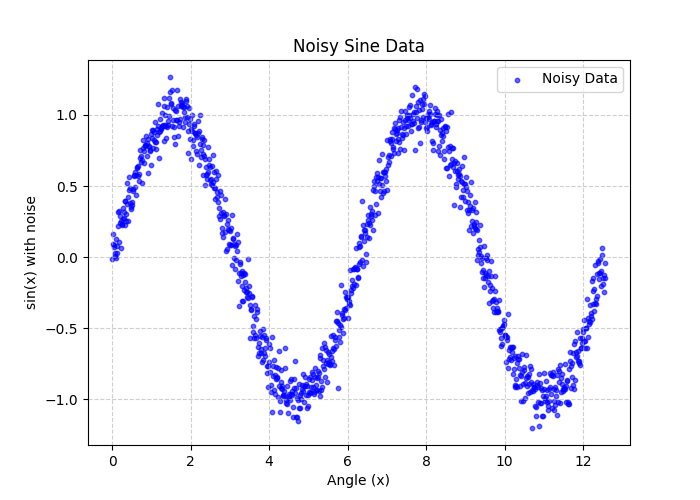
\includegraphics[width=0.8\textwidth]{figures/sine_tests/sine_dataset.png}
     \caption{Plot of the noisy sine dataset}
\end{figure}
\end{center}

\subsection{Stage 1: Grid Search Findings}

\noindent Except for the specific parameter under evaluation during the grid search, the system is initialized with the following default hyperparameters:

\begin{itemize}
    \item \textbf{Quantization Factor ($Q$):} $10$
    \item \textbf{Parameter Range:} $[-20, 20]$
    \item \textbf{Kernel Geometry:} Weight kernels of size $3 \times 3$ and bias kernels of size $3$.
    \item \textbf{Traversal Strides:} Horizontal ($x_s$) and vertical ($y_s$) strides are both set to $2$.
    \item \textbf{Search Constraints:} A maximum of $2000$ iterations.
\end{itemize}
%------------------------------------------------------------------- quantization factor test -------------------------------------------------------------------

\noindent \textbf{Impact of the Quantization Factor}

\noindent Based on the empirical results presented in the accompanying figure, the hyperparameter grid search demonstrated a clear dependency of the final achieved loss on the selected quantization factor, $Q$. Specifically, among the tested values ($Q=10$, $Q=100$, and $Q=1000$), the lower and intermediate factors of $Q=10$ and $Q=100$ yielded the most favorable and comparable outcomes, both achieving a final mean loss of approximately $0.17$. 

In contrast, the highest quantization factor, $Q=1000$, resulted in significantly poorer performance, with a final mean loss of $0.41$. This suggests that while $Q=10$ and $Q=100$ provide a sufficiently discretized weight space for efficient A* traversal, $Q=1000$ leads to a search space that is too fine-grained. At this higher resolution, the distance between meaningful states may hinder the algorithm's ability to reach a global minimum within the allocated iteration budget.

To evaluate the stability and convergence of the proposed methodology, the following results represent the average loss across 10 independent runs for each tested hyperparameter configuration. Figure below provides a clear measure of statistical variability and reproducibility, where the solid lines represent the average loss and the surrounding shaded regions indicate the one standard deviation ($\pm 1\sigma$) interval.

\begin{center}
\begin{figure}[H]
    \centering
    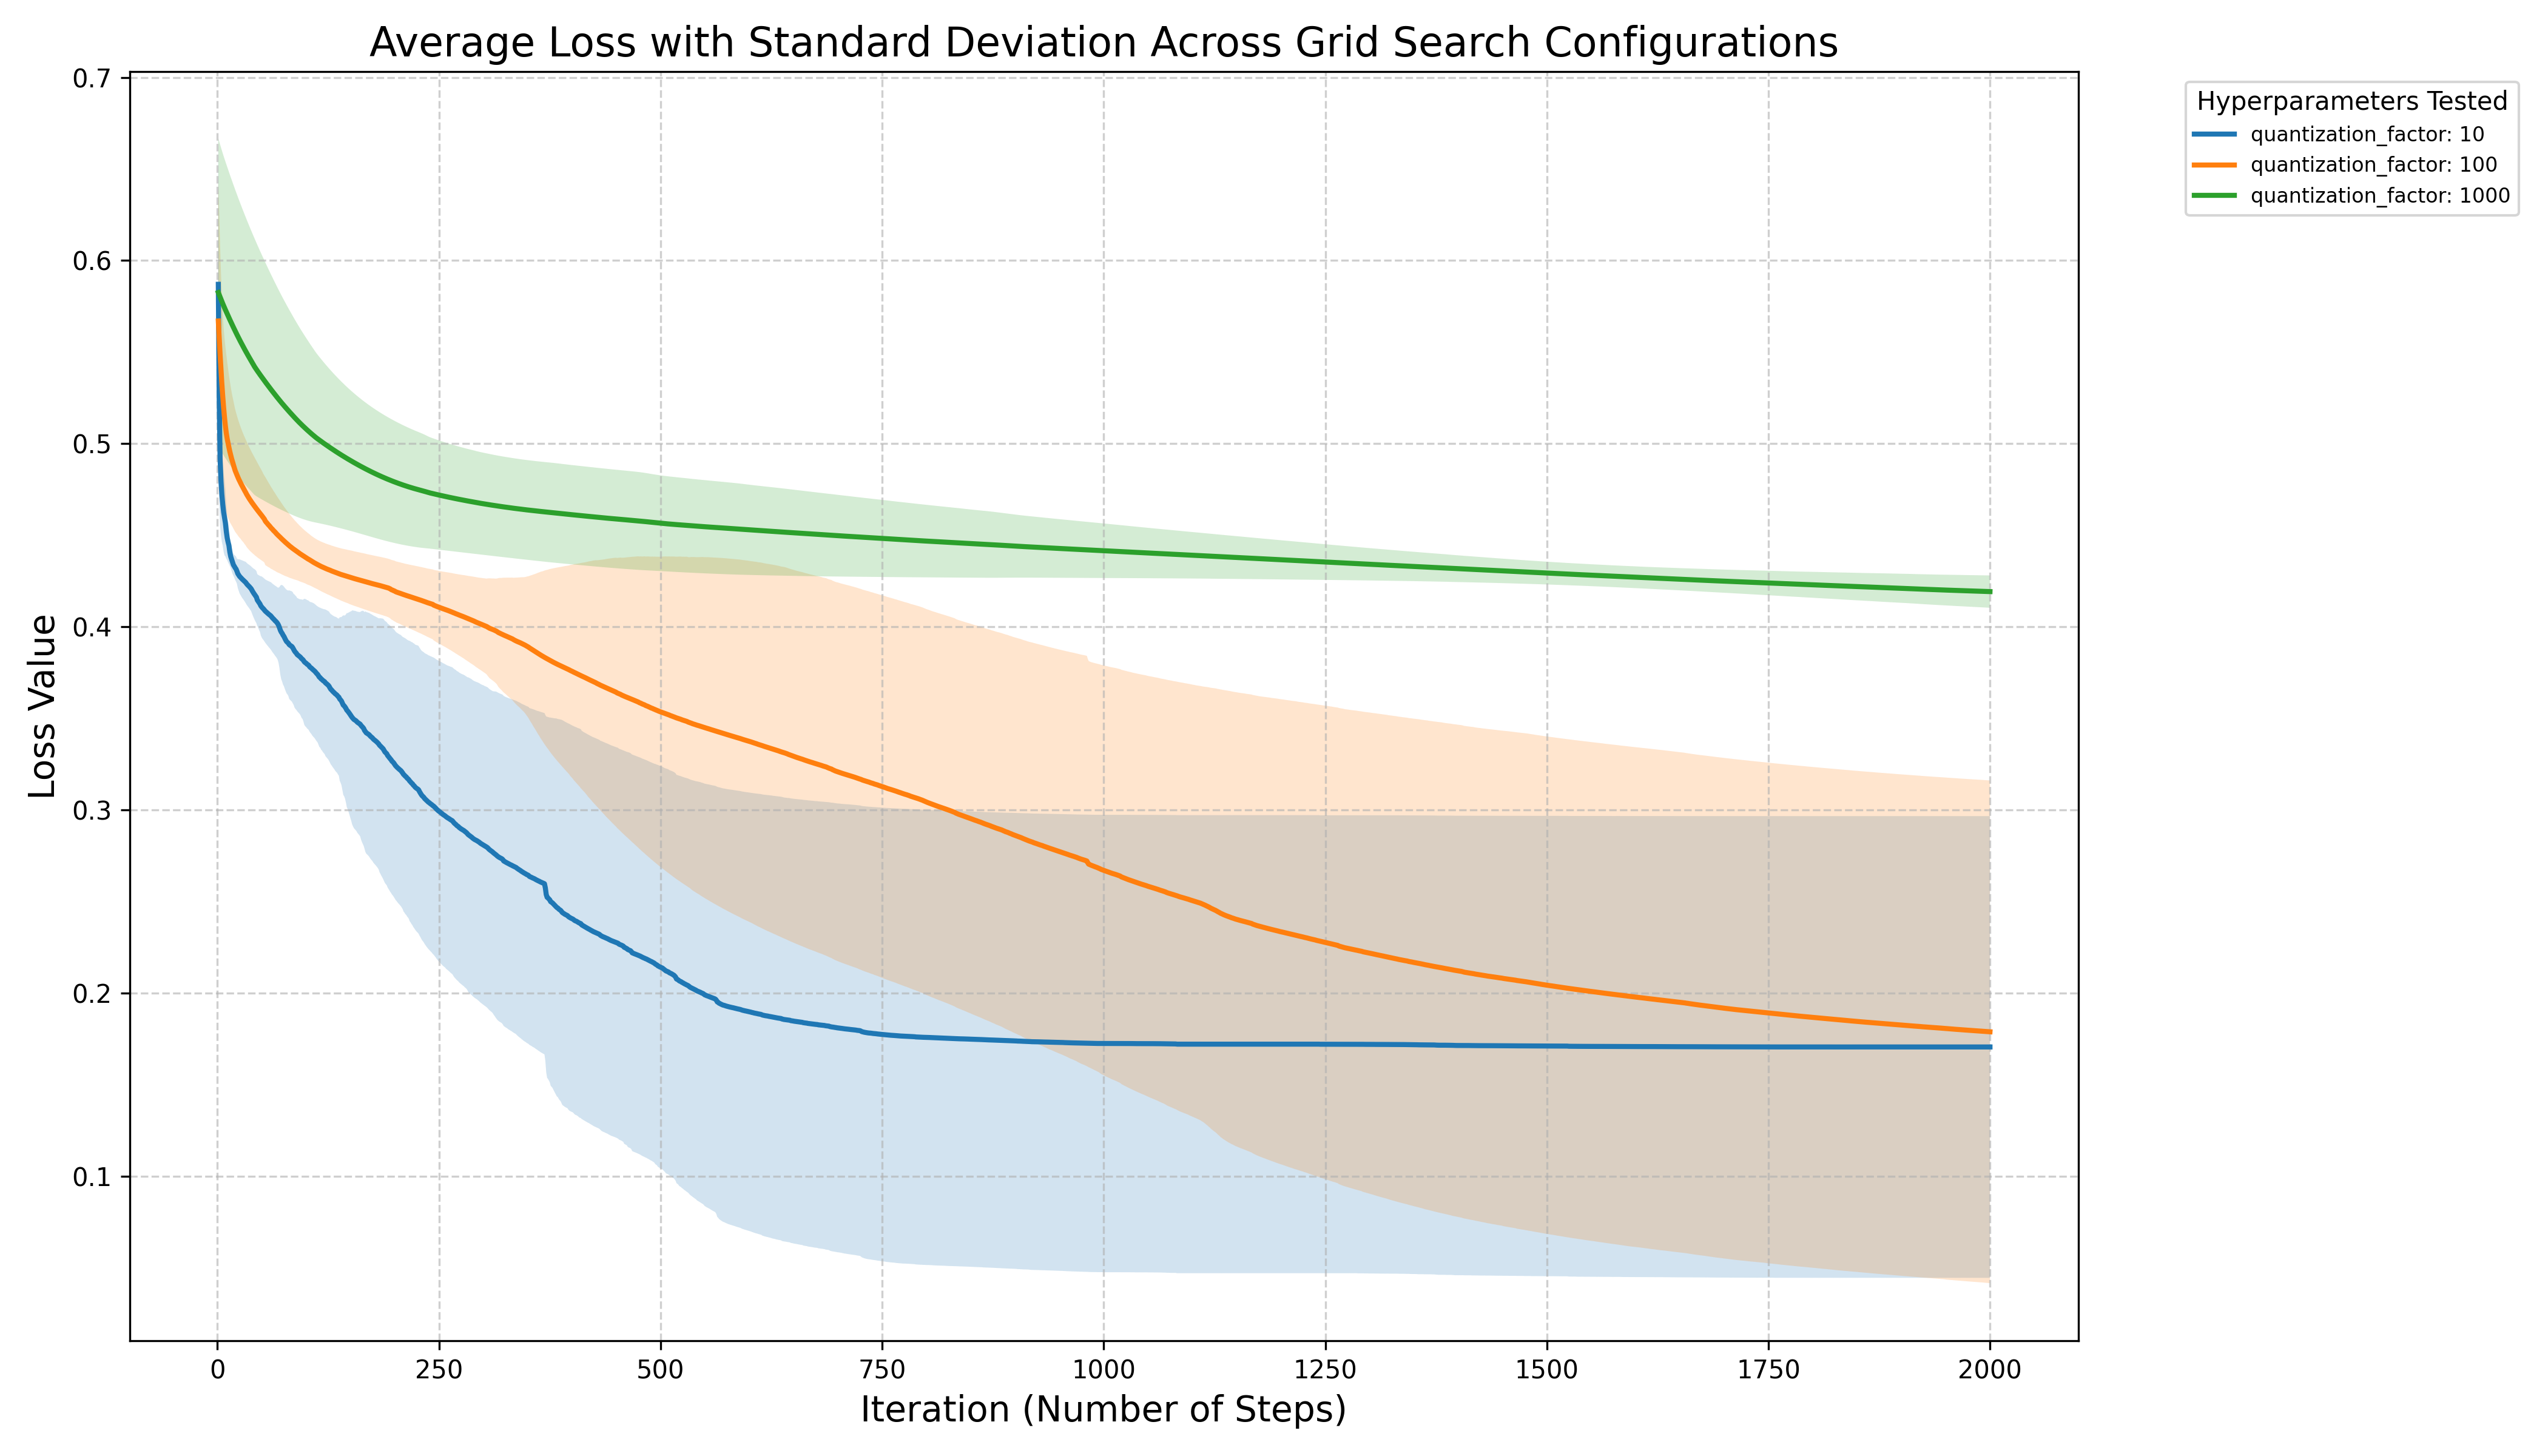
\includegraphics[width=1.1\textwidth]{figures/sine_grid_search/sine_test_quantization_factor_avg_loss.png}
    \caption{Comparison of the mean loss across training iterations for varying quantization factors ($Q \in \{10, 100, 1000\}$)}
\end{figure}
\end{center}


\begin{table}[htbp]
\centering
\caption{Impact of Quantization Factor ($Q$) on Sine Regression Performance}
\label{tab:sine_gs_q_impact}
\resizebox{\textwidth}{!}{%
\begin{tabular}{|c|c|c|c|c|c|c|}
\hline
\textbf{QF ($Q$)} & \textbf{Mean Loss} & \textbf{Median Loss} & \textbf{Std. Dev.} & \textbf{Min Loss} & \textbf{Max Loss} & \textbf{Mean Time (s)} \\
\hline
10 & \textbf{0.1705} & \textbf{0.1049} & 0.1261 & 0.0570 & 0.4328 & \textbf{367.11} \\
100 & 0.1788 & 0.1093 & 0.1373 & \textbf{0.0435} & \textbf{0.3834} & 423.68 \\
1000 & 0.4192 & 0.4222 & \textbf{0.0088} & 0.4018 & 0.4304 & 431.09 \\
\hline
\end{tabular}%
}
\end{table}


%------------------------------------------------------------------- parameter range test -------------------------------------------------------------------
\newpage

\noindent \textbf{Impact of the Network Parameters Range}

\noindent A second set of experiments was conducted to determine the optimal numerical weight range for the network parameters, defining the boundary constraints for the quantized weights. We evaluated three distinct intervals: $[-5, 5]$, $[-10, 10]$, and $[-20, 20]$.

\noindent Analysis of the results demonstrates a non-monotonic trend in performance relative to the range width. The intermediate range of $[-10, 10]$ yielded the best performance, achieving the lowest mean loss of $0.1672$. In comparison, the narrowest range ($[-5, 5]$) resulted in a higher mean loss of $0.2507$, likely due to insufficient model expressiveness. Interestingly, the widest range ($[-20, 20]$) also showed a performance degradation compared to the medium interval, with a mean loss of $0.2100$. 

\noindent These observations suggest that while a range must be broad enough to provide the necessary search capacity, an excessively wide weight space may increase the search complexity. Consequently, the $[-10, 10]$ interval strikes the most effective balance between parameter flexibility and search efficiency for this architecture.

\begin{center}
\begin{figure}[H]
    \centering
    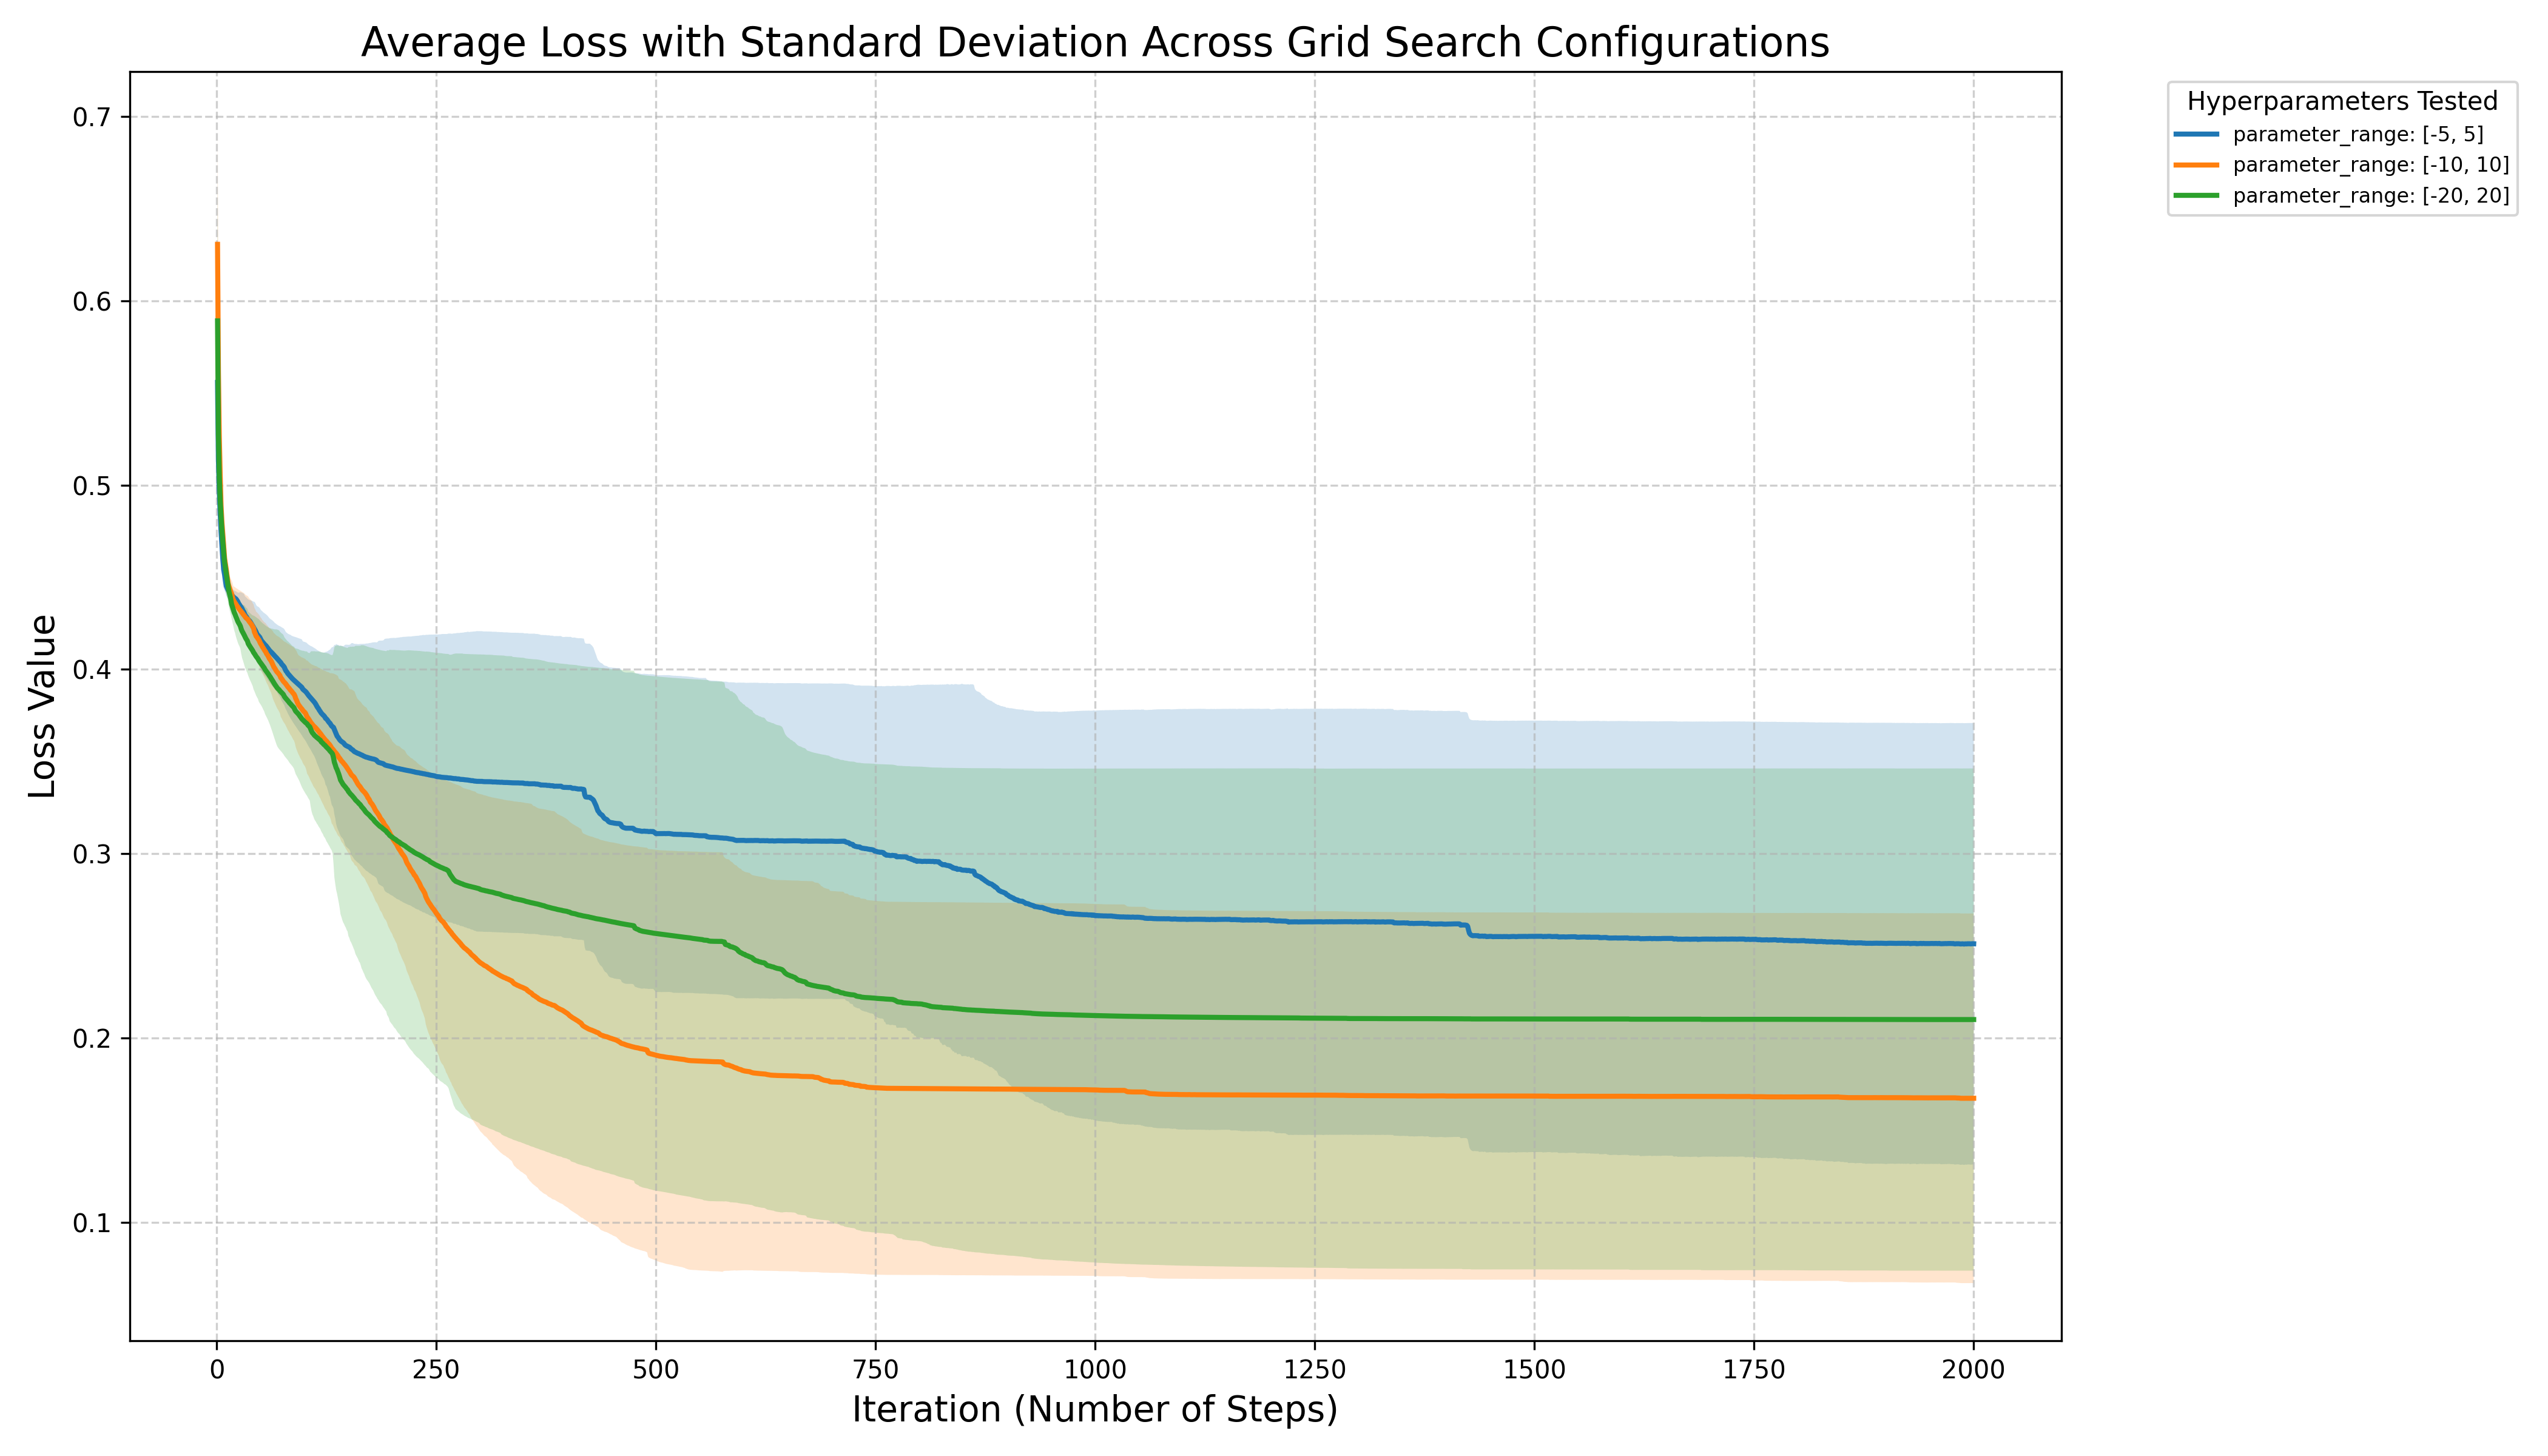
\includegraphics[width=1.2\textwidth]{figures/sine_grid_search/sine_test_parameter_range_avg_loss.png}
    \caption{Comparison of the mean loss across training iterations for varying Parameter Ranges}
\end{figure}
\end{center}


\begin{table}[htbp]
\centering
\caption{Impact of Parameter Range (PR) on Sine Regression Performance}
\label{tab:sine_gs_range_impact}
\resizebox{\textwidth}{!}{%
\begin{tabular}{|c|c|c|c|c|c|c|}
\hline
\textbf{PR} & \textbf{Mean Loss} & \textbf{Median Loss} & \textbf{Std. Dev.} & \textbf{Min Loss} & \textbf{Max Loss} & \textbf{Mean Time (s)} \\
\hline
$[-5, 5]$   & 0.2507 & 0.2666 & 0.1200 & 0.0599 & 0.4259 & \textbf{274.99} \\
$[-10, 10]$ & \textbf{0.1672} & \textbf{0.1456} & \textbf{0.1003} & 0.0618 & 0.3893 & 312.69 \\
$[-20, 20]$ & 0.2100 & 0.2104 & 0.1363 & \textbf{0.0433} & \textbf{0.3717} & 369.17 \\
\hline
\end{tabular}%
}
\end{table}

%------------------------------------------------------------------- max iterations test -------------------------------------------------------------------

\newpage

\noindent \textbf{Effect of Maximum Iterations ($I_{\text{max}}$)}

\noindent The third parameter evaluated was the maximum number of search iterations ($I_{\text{max}}$), testing values of $1,000$ and $2,000$. Unlike fixed-step methodologies, in this framework, $I_{\text{max}}$ acts as a hard cap on the exploration budget within the weight space.

\noindent As demonstrated by the empirical results, the configuration with $I_{\text{max}} = 1,000$ iterations proved to be the most efficient, achieving a mean terminal loss of $0.1789$. Interestingly, doubling the computational budget to $I_{\text{max}} = 2,000$ did not yield a performance gain, instead resulting in a slightly higher mean loss of $0.1884$ and a significant increase in average execution time from approximately $201$ seconds to $348$ seconds.

\noindent This observation suggests that the search typically converges to a stable local minimum within the first $1,000$ iterations. Rather than facilitating the discovery of deeper minima, the extended budget allows the algorithm to persist in high-dimensional plateaus without meaningful improvement.
\begin{center}
\begin{figure}[H]
    \centering
    
\includegraphics[width=1.2\textwidth]{figures/sine_grid_search/sine_test_max_iterations_avg_loss.png}
    \caption{Comparison of the mean loss across training iterations for varying $I_{\text{max}}$ parameter}

\end{figure}
\end{center}


\begin{table}[htbp]
\centering
\caption{Impact of Maximum Iterations on Sine Regression Performance}
\label{tab:sine_gs_iter_impact}
\resizebox{\textwidth}{!}{%
\begin{tabular}{|c|c|c|c|c|c|c|}
\hline
\textbf{Iterations} & \textbf{Mean Loss} & \textbf{Median Loss} & \textbf{Std. Dev.} & \textbf{Min Loss} & \textbf{Max Loss} & \textbf{Mean Time (s)} \\
\hline
\textbf{1000} & \textbf{0.1789} & \textbf{0.1360} & 0.1283 & 0.0380 & 0.3563 & \textbf{201.29} \\
2000 & 0.1884 & 0.1591 & 0.1176 & 0.0566 & 0.3546 & 347.74 \\
\hline
\end{tabular}
}
\end{table}


%\newpage
%------------------------------------------------------------------------------------------------------------------------------------------------------------------

\noindent \textbf{Effect of Kernel Geometry and Traversal Strides}

\noindent A critical set of experiments was conducted to evaluate the influence of the sliding window geometry on search efficiency. We tested four configurations varying the Weight Kernel size ($WK$), Bias Kernel size ($BK$), and the uniform traversal stride ($S$), where horizontal and vertical strides were kept equal ($x_s = y_s = S$). These parameters determine the search graph's branching factor and the 'spatial span' of each transition, effectively governing the extent of weight space coverage per exploration step.

\noindent Analysis of the results indicates that the choice of kernel dimensions significantly impacts the convergence rate and terminal loss. Larger kernels effectively "squash" the search depth by updating more parameters per hop, while the stride regulates the overlap between successive updates. 

\begin{center}
\begin{figure}[H]
    \centering
    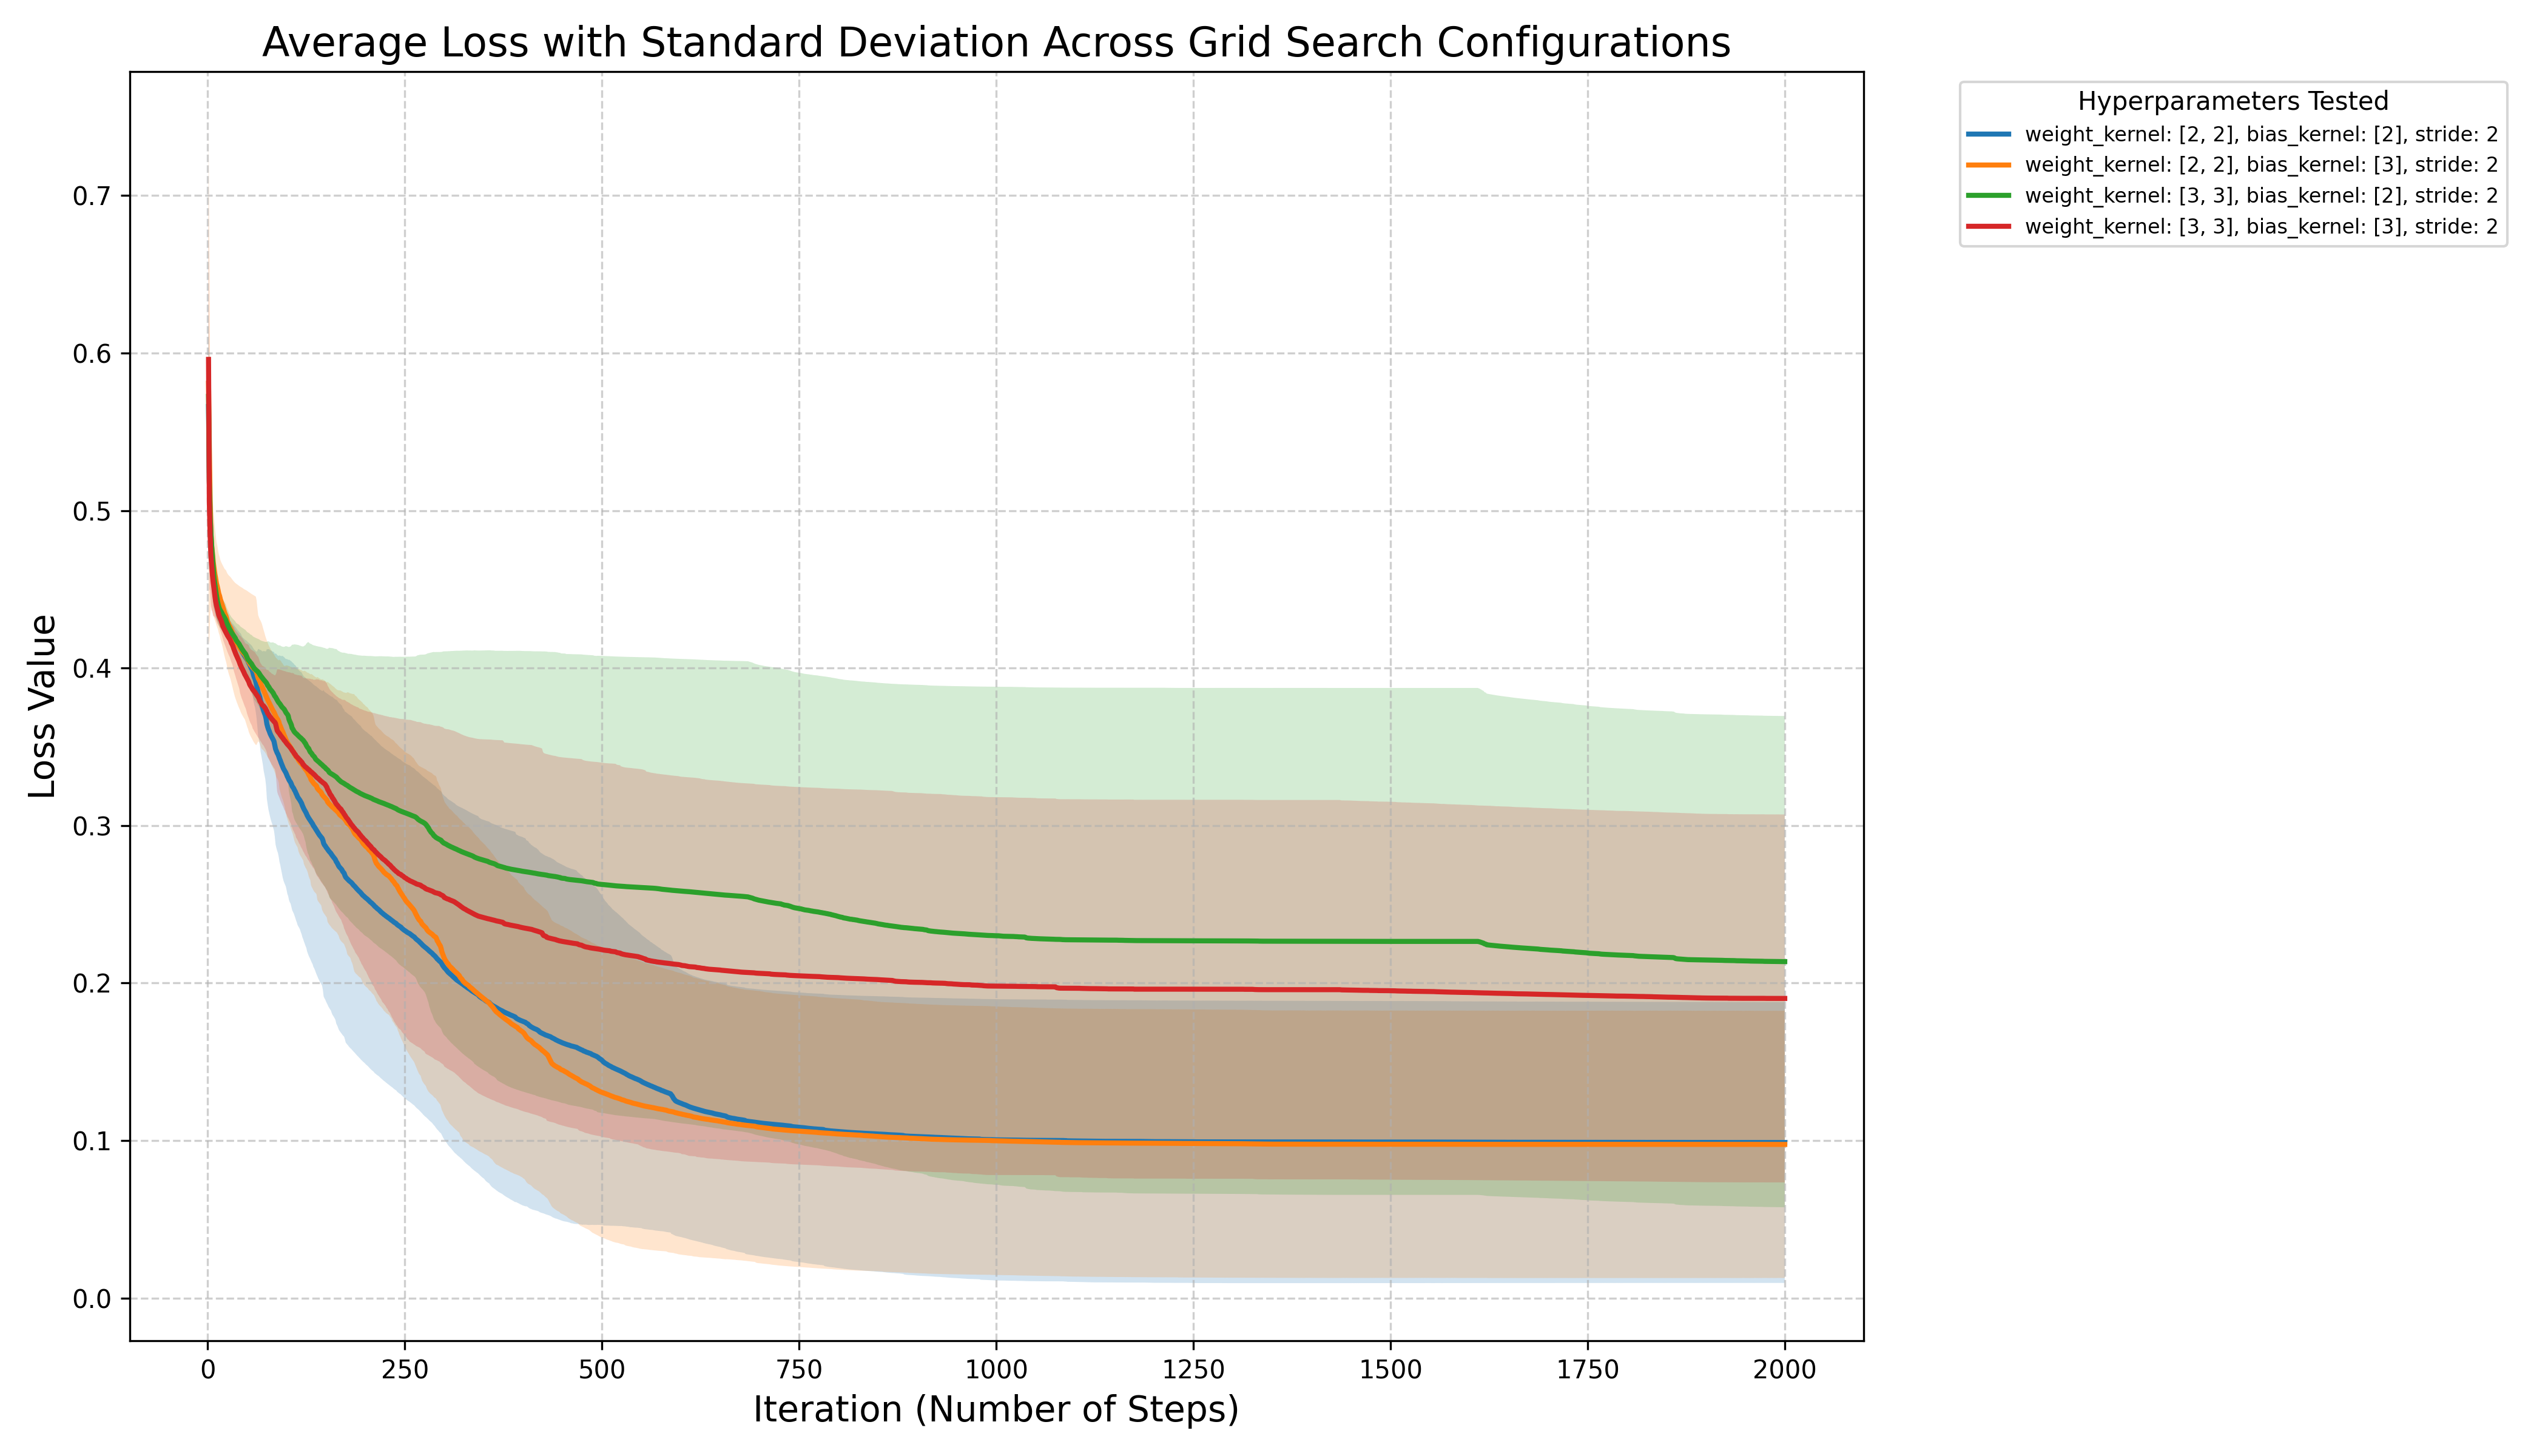
\includegraphics[width=1.2\textwidth]{figures/sine_grid_search/sine_test_kernel_stride_avg_loss.png}
     \caption{Evolution of mean loss across iterations for varying kernel geometries and stride values}
\end{figure}
\end{center}


\begin{table}[htbp]
\centering
\caption{Impact of Kernel Sizes and Strides on Sine Regression Performance}
\label{tab:sine_gs_kernel_impact}
\resizebox{\textwidth}{!}{%
\begin{tabular}{|c|c|c|c|c|c|c|c|c|}
\hline
\textbf{WK} & \textbf{BK} & \textbf{S} & \textbf{Mean Loss} & \textbf{Median Loss} & \textbf{Std. Dev.} & \textbf{Min Loss} & \textbf{Max Loss} & \textbf{Mean Time (s)} \\
\hline
$[2, 2]$ & $[2]$ & 2 & 0.0987 & \textbf{0.0565} & 0.0892 & \textbf{0.0196} & \textbf{0.3134} & 499.99 \\
$[2, 2]$ & $[3]$ & 2 & \textbf{0.0975} & 0.0673 & \textbf{0.0848} & 0.0217 & 0.3199 & 478.15 \\
$[3, 3]$ & $[2]$ & 2 & 0.2136 & 0.1644 & 0.1560 & 0.0505 & 0.4360 & 395.87 \\
$[3, 3]$ & $[3]$ & 2 & 0.1902 & 0.1706 & 0.1168 & 0.0673 & 0.3973 & \textbf{357.17} \\
\hline
\end{tabular}
}
\end{table}

\noindent This structured traversal ensures that the search focuses on localized functional blocks, prioritizing regional weight adjustments. By optimizing these geometric parameters, the algorithm achieves a balance between granular precision and broad exploration, mitigating the computational overhead typically associated with discrete search in high-dimensional spaces.

%------------------------------------------------------------------------------------------------------------------------------------------------------------------

%The optimal hyperparameters selected for the final training (Stage 2) were: $Q=10$, Parameter Range $[-10, 10]$, $\text{param\_fraction}=1.0$, $\text{max\_iterations}=5000$ and $L_{\text{target}}=0.01$.

\subsection{Stage 2 \& 3: Training and Comparative Analysis}

%%%%%%%%%%%%%%%%%%%%%%%%%%%%%%%%%%%%%%%%%%%%%%%%%%%%%%%%%%%%%%%%%%%%%%%%%%%%%%%%%%%%%%%%%%%%%%%%%%%%%%%%%%%%%%%%%%%%%%%%%%%%%%%%%%%%

\noindent \textbf{Explanation of Plots: Statistical Methodology}

\noindent The comparative analysis of A* search and Gradient Descent relies on two complementary visualization techniques, each providing a distinct view of the algorithms' performance across the ten independent runs.

\noindent \textbf{Mean Loss with Standard Deviation Shading}

\noindent The solid line represents the average loss ($\bar{L}$) across all ten runs at every iteration, clearly demonstrating which method achieves faster convergence or reaches a lower loss plateau on average.

\noindent \textbf{Interpretation of Variability (Standard Deviation $\pm 1\sigma$):} The shaded area surrounding the mean line represents the standard deviation ($\pm 1\sigma$) of the loss at each iteration. This is a crucial measure of an algorithm's consistency and robustness.
\begin{itemize}
    \item A narrow shaded band means the method is highly consistent, its performance is reliable and typically near the average, regardless of the random initial weights.
    \item A wide shaded band means the method is volatile ($\sigma$ is large) and highly dependent on the random initialization. A wide band often signals that the algorithm frequently gets stuck in poor local minima or conversely, occasionally finds good solutions.
\end{itemize}

\newpage
\noindent \textbf{Final Loss Box Plot}

\noindent This plot provides a concise summary of the distribution of the final terminal loss achieved by each method after the completion of $I_{\text{max}}$ iterations. It is ideal for comparing the final state quality.

\noindent \textbf{Interpretation of Distribution:}
\begin{itemize}
    \item \textbf{The Median Line:} The horizontal line inside the box shows the median (the 50th percentile) result. The median is a robust measure of typical performance, as it is less sensitive to extreme outliers than the mean.
    \item \textbf{The Box (Interquartile Range, IQR):} The vertical span of the box represents the middle 50\% of your results (from the 25th to the 75th percentile). A very short box indicates high clustering and consistency in the results. If one box is much lower than another, that method is definitively superior in its typical performance range.
    \item \textbf{Whiskers and Dots (Range and Outliers):} The whiskers show the full range of results (excluding outliers), and individual dots beyond the whiskers identify extreme outliers. These elements help to see how often a method results in a failed run or a single exceptional result.
\end{itemize}

%%%%%%%%%%%%%%%%%%%%%%%%%%%%%%%%%%%%%%%%%%%%%%%%%%%%%%%%%%%%%%%%%%%%%%%%%%%%%%%%%%%%%%%%%%%%%%%%%%%%%%%%%%%%%%%%%%%%%%%%%%%%%%%%%%%%


\noindent \textbf{Calculation of Whisker Range and Outliers}

\noindent The length of the whiskers is not arbitrary; it is statistically determined by the data's central spread (the IQR) to identify extreme values (outliers).

\begin{itemize}
    \item \textbf{Interquartile Range (IQR):} This is the length of the box, calculated as $IQR = Q_3 - Q_1$.
    \item \textbf{Whisker Boundaries:} The upper and lower whiskers extend to the most extreme data points that are no more than $\mathbf{1.5 \times IQR}$ away from the box edges. The boundaries are formally defined as:
    $$
    \text{Upper Bound} = Q_3 + 1.5 \times IQR
    $$
    $$
    \text{Lower Bound} = Q_1 - 1.5 \times IQR
    $$
    \item \textbf{Outliers:} Any final loss value that falls outside these calculated bounds is considered an outlier and is plotted as an individual point (dot). In the context of loss, points above the upper whisker represent runs where the algorithm performed significantly worse than its typical operation.
\end{itemize}

%%%%%%%%%%%%%%%%%%%%%%%%%%%%%%%%%%%%%%%%%%%%%%%%%%%%%%%%%%%%%%%%%%%%%%%%%%%%%%%%%%%%%%%%%%%%%%%%%%%%%%%%%%%%%%%%%%%%%%%%%%%%%%%%%%%%

\subsection{Comparison with Gradient Descent: $I_{\text{max}} = 1,000$}

\noindent To quantitatively assess the performance of the A* search approach against the established optimization method of Gradient Descent (GD) on the sine dataset, a comparative study was conducted. Both A* and GD were executed for $I_{\text{max}}=1,000$ training steps. To ensure robustness, ten independent runs ($n=10$) were performed for each algorithm, starting from different random weight initializations. The statistical results are summarized in Table \ref{tab:1k_stats}, and the performance trajectory is presented in the following figures.

\begin{center}
\begin{figure}[H]
    \centering
    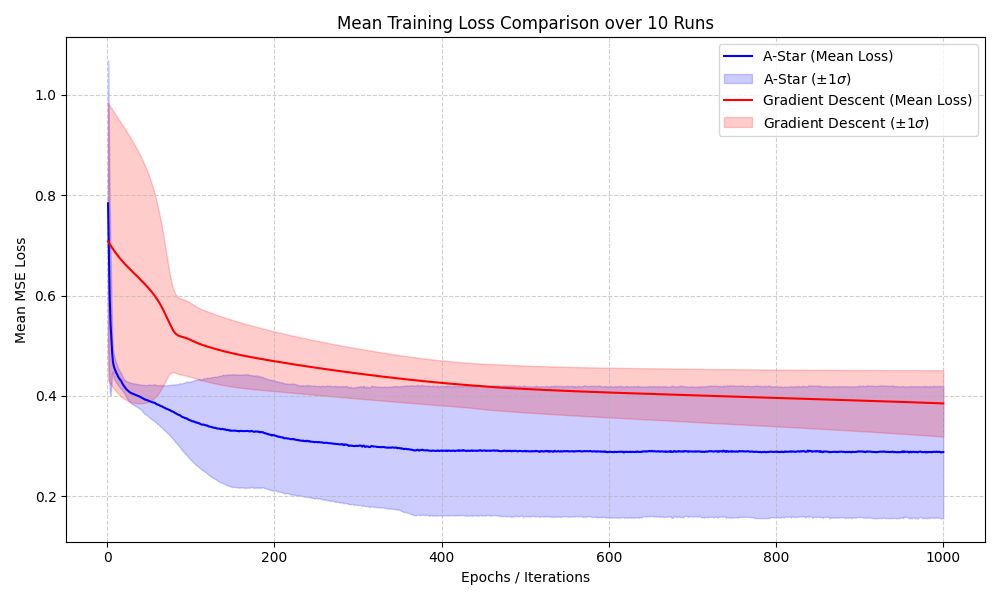
\includegraphics[width=1.0\textwidth]{figures/sine_tests/mean_loss_comparison_with_std_1k.png}
     \caption{Mean Loss Trajectory with Standard Deviation Shading for $I_{\text{max}}=\text{1,000}$ Iterations. This plot illustrates the average loss over ten independent runs for both A* Search (Novel) and Gradient Descent (Classic), with the shaded region representing $\pm 1$ standard deviation. It highlights convergence speed and the consistency of each algorithm's performance over time.}
\end{figure}
\end{center}

\begin{center}
\begin{figure}[H]
    \centering
    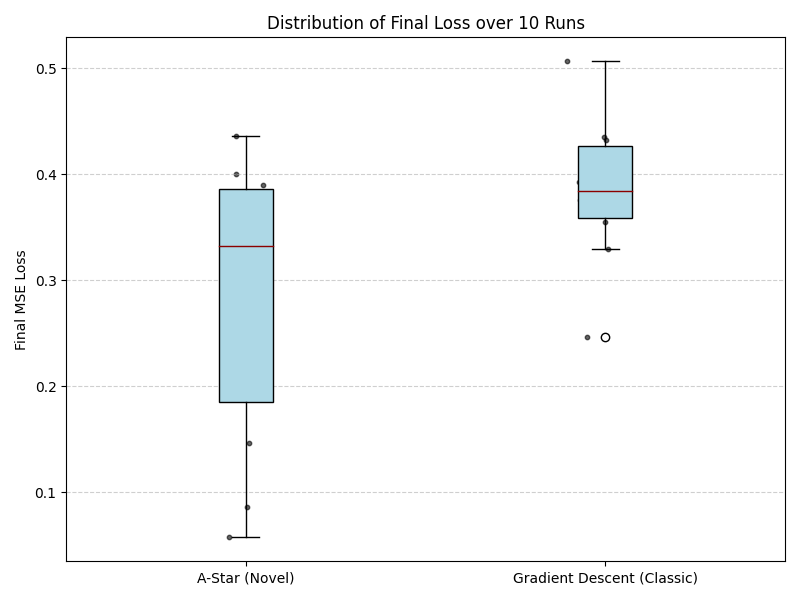
\includegraphics[width=1.0\textwidth]{figures/sine_tests/final_loss_boxplot_1k.png}
     \caption{Final Loss Box Plot for $I_{\text{max}}=\text{1,000}$ Iterations. This box plot summarizes the distribution of the terminal loss values achieved by A* Search (Novel) and Gradient Descent (Classic) over ten independent runs. The box represents the interquartile range (IQR), the central line indicates the median, and whiskers show the range of results (excluding outliers).}
\end{figure}
\end{center}

\begin{table}[H]
    \centering
    \caption{Comparative Statistics Over Ten Runs for $I_{\text{max}}=1,000$ Iterations}
    \label{tab:1k_stats}
    \begin{tabular}{|l|c|c|}
        \hline
        \textbf{Metric} & \textbf{A* Search (Novel)} & \textbf{Gradient Descent (Classic)} \\
        \hline
        Average Loss ($\bar{L}$) & \textbf{0.285213} & 0.385243 \\
        Median Loss & \textbf{0.331870} & 0.384283 \\
        Standard Deviation ($\sigma$) & 0.130934 & \textbf{0.066165} \\
        Variance ($\sigma^2$) & 0.017144 & \textbf{0.004378} \\
        Minimum Loss ($L_{\min}$) & \textbf{0.057494} & 0.246618 \\
        Maximum Loss ($L_{\max}$) & \textbf{0.436191} & 0.506505 \\
        Average Training Time (s) & 100.10 & \textbf{10.20} \\
        \hline
    \end{tabular}
\end{table}

\subsection*{Statistical and Trajectory Analysis}

\noindent \textbf{Performance (Average Loss):} For the $1,000$-iteration budget, the A* search method significantly outperformed GD in terms of central tendency. The A* Average Loss ($\bar{L} = 0.2852$) is substantially lower than the GD Average Loss ($\bar{L} = 0.3852$), a difference of nearly $0.1$ units. This is further supported by the Median Loss, where A* is also clearly superior, indicating that A* typically converges to a better solution within this short number of search iteration.

\noindent \textbf{Best-Case Potential:} A* demonstrated a superior capacity to locate deep minima, achieving a Minimum Loss ($L_{\min} = 0.0575$) that is four times better than GD's best run ($L_{\min} = 0.2466$). This highlights A*'s effective, albeit non-admissible, exploration strategy in the quantized space.

\noindent \textbf{Consistency Trade-off:} The major point of contrast is in solution stability. The Standard Deviation of A* ($\sigma = 0.1309$) is nearly double that of GD ($\sigma = 0.0662$). This indicates that while A* can find much better solutions, its final performance is less consistent and more dependent on the random initialization than Gradient Descent over these $1,000$ steps. The narrow shaded band for GD in the previous plot confirms its superior stability, while the wider band for A* reflects its volatility.

\noindent \textbf{Conclusion for $I_{\text{max}}=1,000$:} Over a short budget of $1,000$ iterations, the A* training framework proves to be the performance leader for the sine regression task, achieving significantly lower average loss, median loss, and minimum loss values than Gradient Descent. While A* introduces a consistency trade-off (higher volatility) compared to the more stable GD, its enhanced capacity to locate superior global solutions in the quantized weight space makes it the preferred method for finding better result.

%%%%%%%%%%%%%%%%%%%%%%%%%%%%%%%%%%%%%%%%%%%%%%%%%%%%%%%%%%%%%%%%%%%%%%%%%%%%%%%%%%%%%%%%%%%%%%%%%%%%%%%%%%%%%%%%%%%%%%%%%%%%%%%%%%%%%%%%%%%%%%%%%%
\subsection{Comparison with Gradient Descent: $I_{\text{max}} = 2,000$}

\noindent To evaluate the mid-term behavior of both A* search and Gradient Descent, the comparative study was conducted using a computational budget of $I_{\text{max}}=2,000$ steps. Ten independent runs ($n=10$) were executed for each method to ensure statistical relevance. The results are summarized in Table \ref{tab:2k_stats}, followed by an analysis of the performance metrics.

\begin{center}
\begin{figure}[H]
    \centering
    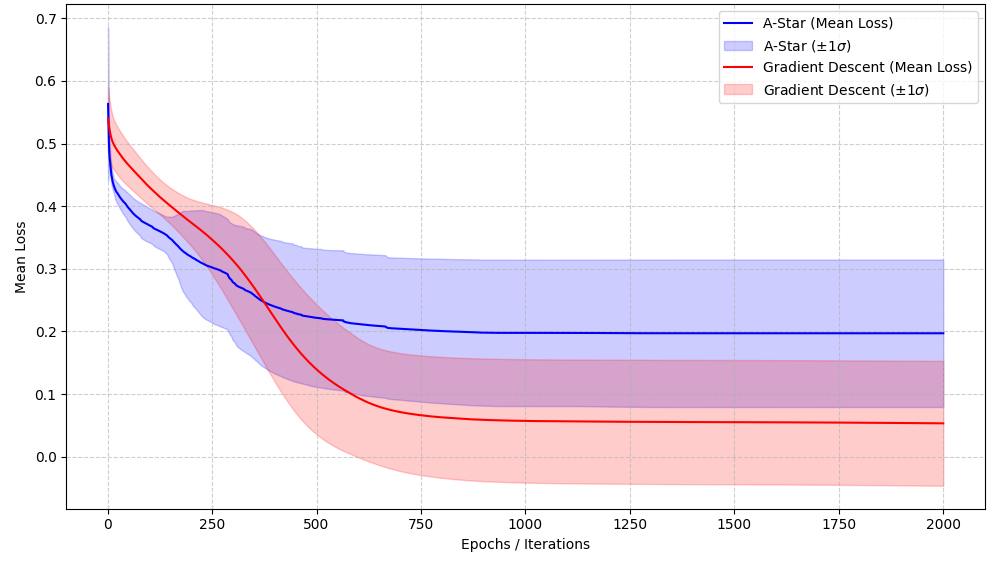
\includegraphics[width=1.0\textwidth]{figures/sine_tests/sine_mean_loss_comparison_with_std_2k.png}
     \caption{Mean Loss Trajectory with Standard Deviation Shading for $I_{\text{max}}=\text{2,000}$ Iterations. This plot illustrates the average loss over ten independent runs for both A* Search and Gradient Descent.}
\end{figure}
\end{center}

\begin{center}
\begin{figure}[H]
    \centering
    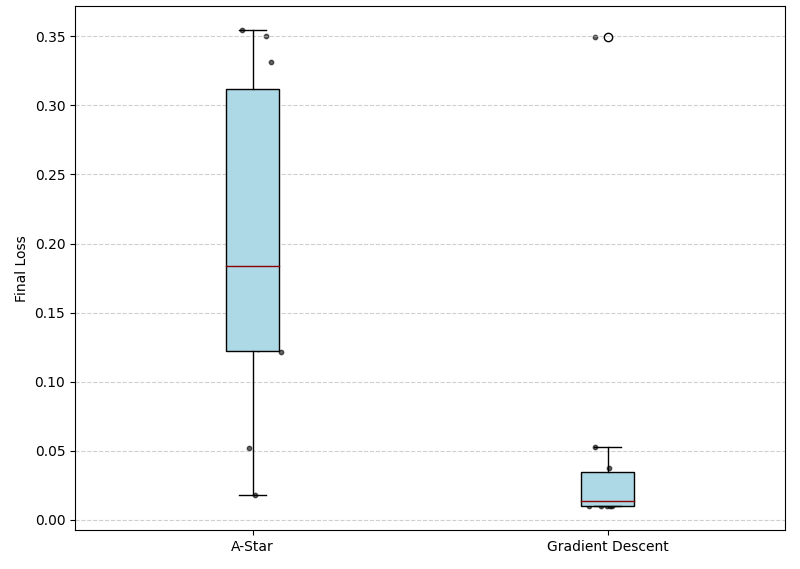
\includegraphics[width=1.0\textwidth]{figures/sine_tests/sine_final_loss_distribution_comparison_2k.png}
     \caption{Final Loss Box Plot for $I_{\text{max}}=\text{2,000}$ Iterations. The plot summarizes the distribution of terminal loss values.}
\end{figure}
\end{center}

\begin{table}[H]
    \centering
    \caption{Comparative Statistics Over Ten Runs for $I_{\text{max}}=2,000$ Iterations}
    \label{tab:2k_stats}
    \begin{tabular}{|l|c|c|}
        \hline
        \textbf{Metric} & \textbf{A* Search} & \textbf{Gradient Descent} \\
        \hline
        Average Loss ($\bar{L}$) & 0.197100 & \textbf{0.053283} \\
        Median Loss & 0.183644 & \textbf{0.013862} \\
        Standard Deviation ($\sigma$) & 0.117757 & \textbf{0.099745} \\
        Variance ($\sigma^2$) & 0.013867 & \textbf{0.009949} \\
        Minimum Loss ($L_{\min}$) & 0.017940 & \textbf{0.009764} \\
        Maximum Loss ($L_{\max}$) & 0.354409 & \textbf{0.349630} \\
        Average Training Time (s) & 453.53 & \textbf{18.07} \\
        \hline
    \end{tabular}
\end{table}

\subsection*{Statistical and Trajectory Analysis}

\noindent \textbf{Dominance in Performance:} At the $2,000$ iteration mark, Gradient Descent exhibits a clear performance lead in terms of central tendency. The average loss for GD ($\bar{L} = 0.0533$) is significantly lower than that of A* ($\bar{L} = 0.1971$). The disparity in Median Loss ($0.0139$ for GD vs. $0.1836$ for A*) further suggests that GD more frequently reaches a high-precision state within this specific computational window.

\noindent \textbf{Convergence and Best-Case Performance:} When examining the peak potential of both algorithms, the results are remarkably competitive. GD achieved a Minimum Loss of $L_{\min} = 0.0098$, while A* followed closely with $L_{\min} = 0.0179$. This comparison indicates that both methods are capable of identifying high-quality solutions; while GD’s continuous gradient exploitation gives it a slight edge in refinement, A* demonstrates that its heuristic search can successfully navigate to the same neighborhood of the global minimum.

\noindent \textbf{Reliability and Variance:} The consistency of the two methods is quite comparable at this scale. GD maintains a Standard Deviation of $\sigma = 0.0997$, which is only slightly lower than the $\sigma = 0.1178$ recorded for A*. This narrow margin suggests that both algorithms offer a similar level of reliability across independent runs. The small difference indicates that A* remains a robust contender in terms of stability.

\noindent \textbf{Computational Efficiency:} There remains a significant difference in computational overhead. GD completed the training in an average of $18.07$ seconds, whereas A* required $453.53$ seconds. This $25\times$ speed advantage for the classic approach highlights the current efficiency of gradient-based updates compared to the more memory-intensive node expansion process inherent in A* search.

\noindent \textbf{Conclusion for $I_{\text{max}}=2,000$:} At $2,000$ iterations, Gradient Descent proves to be highly efficient, offering a lower average loss and faster execution. However, the A* method remains a novel alternative; it achieves a minimum loss and a level of statistical consistency (standard deviation) that are comparable with the classic approach. While A* currently requires more time to process its search space, its ability to reach competitive high-quality solutions suggests significant potential for the heuristic-driven framework.
\newpage

%%%%%%%%%%%%%%%%%%%%%%%%%%%%%%%%%%%%%%%%%%%%%%%%%%%%%%%%%%%%%%%%%%%%%%%%%%%%%%%%%%%%%%%%%%%%%%%%%%%%%%%%%%%%%%%%%%%%%%%%%%%%%%%%%%%%%%%%%%%%%%%%%%%%%%%%%%%%%%%%%%%%%%%%%%%%%%
%-------------------------------------------------------------------    IRIS DATASET -----------------------------------------------------------------------------------------
%%%%%%%%%%%%%%%%%%%%%%%%%%%%%%%%%%%%%%%%%%%%%%%%%%%%%%%%%%%%%%%%%%%%%%%%%%%%%%%%%%%%%%%%%%%%%%%%%%%%%%%%%%%%%%%%%%%%%%%%%%%%%%%%%%%%%%%%%%%%%%%%%%%%%%%%%%%%%%%%%%%%%%%%%%%%%%


\section{Classic Dataset: Iris Flower Classification}
\label{sec:iris_classification}

\noindent The second experiment applies the A* training framework to a classic classification task, assessing its ability to perform MLP parameter optimization in a well known dataset.

\subsection{Dataset and Objective}

The experiment utilizes the canonical Iris dataset, which consists of $150$ samples of three species of Iris flowers (Setosa, Versicolor, Virginica), based on four key features.

\begin{itemize}
    \item \textbf{Input ($x$):} 4 features (sepal length, sepal width, petal length, petal width) standardized to a common scale.
    \item \textbf{Output ($y$):} Three classes (species), encoded using one-hot encoding (e.g., $[1, 0, 0]$ for Setosa).
\item \textbf{MLP Architecture:} Input (4 neurons) $\rightarrow$ 
      Hidden Layer 1 (8 neurons, ReLU) $\rightarrow$ 
      Hidden Layer 2 (16 neurons, ReLU) $\rightarrow$ 
      Hidden Layer 3 (8 neurons, ReLU) $\rightarrow$ 
      Output (3 neurons).\end{itemize}

\noindent The network's task is a three-class classification, aiming to learn the mapping from the four physical measurements to the correct species, minimizing the Categorical Cross-Entropy loss. The performance comparison between A* and Gradient Descent will be primarily evaluated based on this loss function.

\subsection{Stage 1: Optimal Hyperparameters}

\noindent Given the architectural similarities between the sine regression model and the Iris classification model, the optimal hyperparameters found during the sine experiment were adopted for the final comparison phase of the Iris dataset:
\begin{itemize}
    \item \textbf{Quantization Factor:} $Q=10$
    \item \textbf{Parameter Range:} $[-10, 10]$
    \item \textbf{Kernels Shape and Stride:} $ \text{Weight\_kernel}=(2,2), \text{Bias\_kernel}=(2,1) \text{ and Stride}=2$
\end{itemize}


\subsection{Stage 2 \& 3: Training and Comparative Analysis}

\noindent The methodology for visualization and statistical analysis remains identical to that employed for the sine dataset (see Section \ref{sec:sine_regression}, Stage 2 \& 3). The comparison between A* and Gradient Descent is performed over ten independent runs ($n=10$) for two iteration budgets: $I_{\text{max}}=1,000$ and $I_{\text{max}}=2,500$. The same Mean Loss with Standard Deviation Shading and Final Loss Box Plot visualizations are utilized.


%===================================== 1k iterations %=====================================

\subsection{Comparison with Gradient Descent: $I_{\text{max}} = 1,000$}

\noindent The comparative study between A* and GD was first executed with a budget of $I_{\text{max}}=1,000$ steps to assess performance under time constraints. The statistical results are summarized in Table \ref{tab:iris_1k_stats}, and the performance trajectory is presented in the following figures.

\begin{center}
\begin{figure}[H]
    \centering
    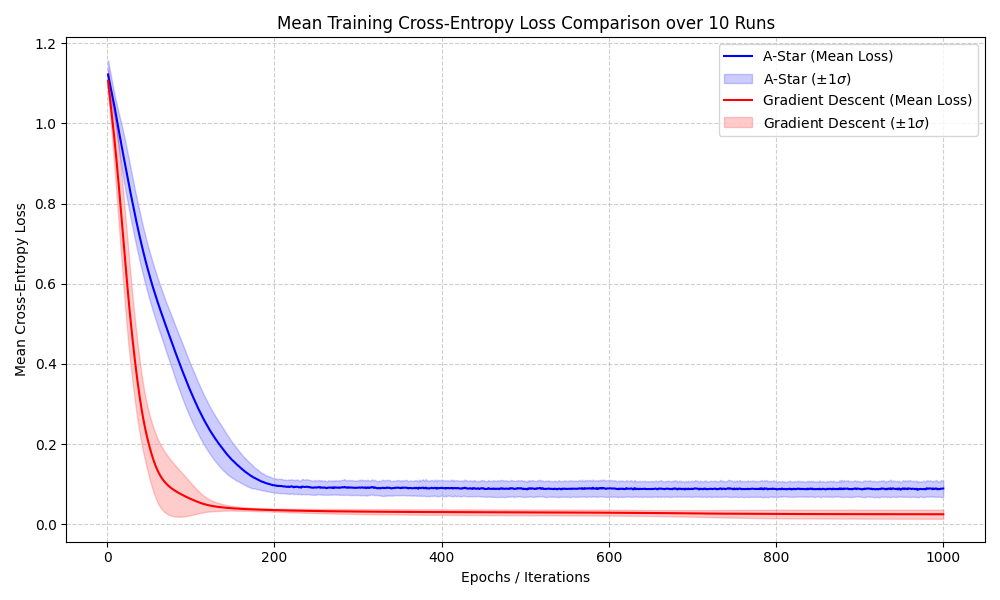
\includegraphics[width=1.0\textwidth]{figures/iris_tests/iris_mean_loss_comparison_with_std_1k.png}
     \caption{Mean Loss Trajectory with Standard Deviation Shading for $I_{\text{max}}=\text{1,000}$ Iterations (Iris Dataset). This plot illustrates the average loss over ten independent runs, highlighting convergence and consistency.}
\end{figure}
\end{center}

\begin{center}
\begin{figure}[H]
    \centering
    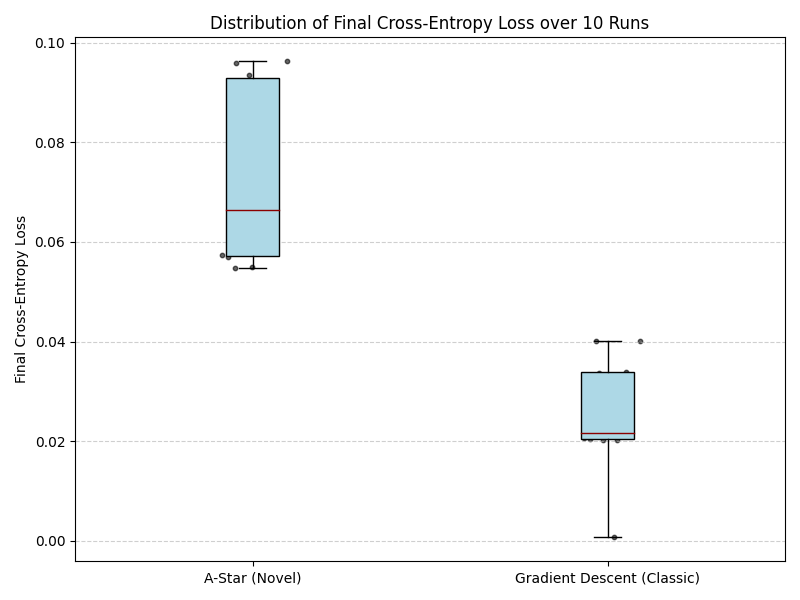
\includegraphics[width=1.0\textwidth]{figures/iris_tests/iris_final_loss_boxplot_1k.png}
     \caption{Final Loss Box Plot for $I_{\text{max}}=\text{1,000}$ Iterations (Iris Dataset). This plot summarizes the distribution of the terminal loss values achieved by both search methods.}
\end{figure}
\end{center}

\begin{table}[H]
    \centering
    \caption{Comparative Statistics Over Ten Runs for $I_{\text{max}}=1,000$ Iterations (Iris Dataset)}
    \label{tab:iris_1k_stats}
    \begin{tabular}{|l|c|c|}
        \hline
        \textbf{Metric} & \textbf{A* Search (Novel)} & \textbf{Gradient Descent (Classic)} \\
        \hline
        Average Loss ($\bar{L}$) & 0.073372 & \textbf{0.025271} \\
        Median Loss & 0.066387 & \textbf{0.021674} \\
        Standard Deviation ($\sigma$) & 0.017490 & \textbf{0.011363} \\
        Variance ($\sigma^2$) & 0.000306 & \textbf{0.000129} \\
        Minimum Loss ($L_{\min}$) & 0.054803 & \textbf{0.000643} \\
        Maximum Loss ($L_{\max}$) & 0.096308 & \textbf{0.040051} \\
        Average Training Time (s) & 336.449361 & \textbf{2.003290} \\
        \hline
    \end{tabular}
\end{table}

\subsection*{Statistical and Trajectory Analysis}

\noindent \textbf{Performance Dominance:} For the $1,000$ iterations on the Iris dataset, Gradient Descent exhibits decisive superiority across all metrics compared to the A* search framework. The GD Average Loss ($\bar{L} = 0.0253$) is nearly three times lower than the A* Average Loss ($\bar{L} = 0.0734$), and its Median Loss is also significantly better. This indicates that the continuous optimization landscape is highly efficient for GD even in short runs.

\noindent \textbf{Best-Case and Consistency:} GD demonstrates superior performance potential, achieving a minimum loss ($L_{\min} = 0.0006$) which is two orders of magnitude better than the A* minimum ($L_{\min} = 0.0548$). Furthermore, GD is also significantly more consistent; its Standard Deviation ($\sigma = 0.0114$) and Variance are lower than A*'s ($\sigma = 0.0175$). This means that GD not only finds better solutions on average but does so more reliably.

\noindent \textbf{Computational Efficiency:} The vast difference in computational time is also notable. GD completes the $1,000$ iterations in approximately 2.00 seconds, whereas the A* search requires over 336 seconds due to the overhead of neighbor generation, heuristic evaluation, and priority queue management.

\noindent \textbf{Conclusion for $I_{\text{max}}=1,000$:} For this specific classification task and short budget, the highly constrained, non-admissible A* search in the quantized weight space is ineffective. GD benefits greatly from the well-behaved continuous optimization surface, resulting in demonstrably better performance, higher consistency, and significantly faster training time.


%===================================== 2k iterations %===================================== 
\subsection{Comparison with Gradient Descent: $I_{\text{max}} = 2,000$}

\noindent The comparative study was extended to $I_{\text{max}}=2,000$ steps to evaluate the convergence behavior of both methods on the Iris dataset. The statistical results across ten independent runs are presented in Table \ref{tab:iris_2k_stats}, followed by an analysis of the performance metrics and stability.

\begin{center}
\begin{figure}[H]
    \centering
    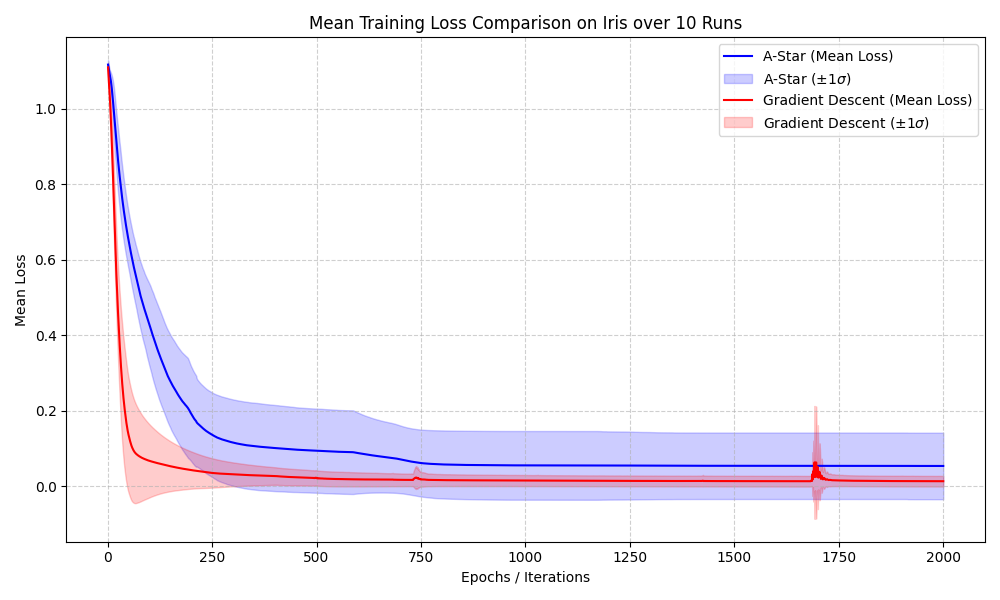
\includegraphics[width=1.0\textwidth]{figures/iris_tests/iris_mean_loss_comparison_with_std_2k.png}     
     \caption{Mean Loss Trajectory with Standard Deviation Shading for $I_{\text{max}}=\text{2,000}$ Iterations (Iris Dataset). This plot illustrates the average loss over ten independent runs, highlighting the convergence speed of both search methods.}
\end{figure}
\end{center}

\begin{center}
\begin{figure}[H]
    \centering
    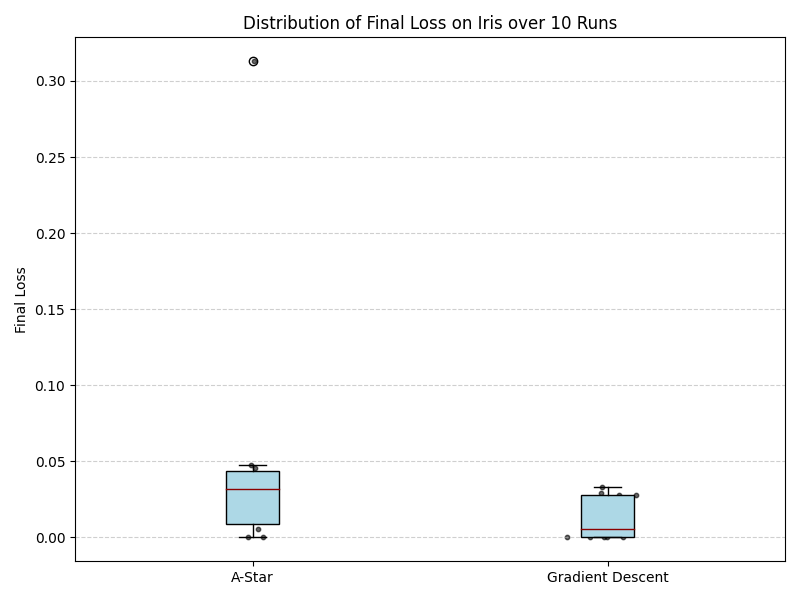
\includegraphics[width=1.0\textwidth]{figures/iris_tests/iris_final_loss_boxplot_2k.png}    
     \caption{Final Loss Box Plot for $I_{\text{max}}=\text{2,000}$ Iterations (Iris Dataset). This plot summarizes the distribution of the terminal loss values achieved by A* and Gradient Descent.}
\end{figure}
\end{center}

\begin{table}[H]
    \centering
    \caption{Comparative Statistics Over Ten Runs for $I_{\text{max}}=2,000$ Iterations (Iris Dataset)}
    \label{tab:iris_2k_stats}
    \begin{tabular}{|l|c|c|}
        \hline
        \textbf{Metric} & \textbf{A* Search} & \textbf{Gradient Descent} \\
        \hline
        Average Loss ($\bar{L}$) & 0.053327 & \textbf{0.012917} \\
        Median Loss & 0.031683 & \textbf{0.005256} \\
        Standard Deviation ($\sigma$) & 0.088180 & \textbf{0.014070} \\
        Variance ($\sigma^2$) & 0.007776 & \textbf{0.000198} \\
        Minimum Loss ($L_{\min}$) & 0.000272 & \textbf{0.000005} \\
        Maximum Loss ($L_{\max}$) & 0.313026 & \textbf{0.033427} \\
        Average Training Time (s) & 469.12 & \textbf{4.90} \\
        \hline
    \end{tabular}
\end{table}

\subsection*{Statistical and Trajectory Analysis}

\noindent \textbf{Dominance in Performance:} At the $2,000$ iteration mark, Gradient Descent (GD) exhibits a clear performance lead in terms of central tendency on the Iris dataset. The average loss for GD ($\bar{L} = 0.0129$) is significantly lower than that of A* ($\bar{L} = 0.0533$). The disparity in Median Loss ($0.0053$ for GD vs. $0.0317$ for A*) further suggests that GD more frequently reaches a high-precision state within this specific computational window for classification tasks.

\noindent \textbf{Convergence and Best-Case Performance:} When examining the peak potential of both algorithms, the results are remarkably competitive and showcase high precision. GD achieved a Minimum Loss of $L_{\min} = 0.000005$, while A* followed with an impressive $L_{\min} = 0.000272$. This comparison indicates that both methods are highly capable of identifying optimal solutions; while GD’s exploitation of the continuous loss surface allows for extreme refinement, A* demonstrates that its heuristic search can successfully navigate to a nearly identical neighborhood of the global minimum.

\noindent \textbf{Reliability and Variance:} The consistency of the two methods shows a wider margin in this scenario, though both remain within a stable range. GD maintains a Standard Deviation of $\sigma = 0.0141$, while A* recorded a $\sigma = 0.0882$. While GD is more consistent at this scale, the low absolute value of the A* variance suggests it remains a robust contender in terms of stability.

\noindent \textbf{Computational Efficiency:} There remains a significant difference in computational overhead. GD completed the training in an average of $4.90$ seconds, whereas A* required $469.12$ seconds. This speed advantage for the classic approach highlights the current efficiency of gradient-based updates compared to the more memory-intensive and computationally demanding node expansion process inherent in the A* search framework.

\noindent \textbf{Conclusion for $I_{\text{max}}=2,000$:} At $2,000$ iterations, Gradient Descent proves to be highly efficient for the Iris task, offering a lower average loss and near-instant execution. While A* currently requires more time to process its search space and exhibits higher variance, its ability to locate high-precision solutions confirms the significant potential of heuristic-driven frameworks in neural network optimization.
%%%%%%%%%%%%%%%%%%%%%%%%%%%%%%%%%%%%%%%%%%%%%%%%%%%%%%%%%%%%%%%%%%%%%%%%%%%%%%%%%%%%%%%%%%%%%%%%%%%%%%%%%%%%%%%%%%%%%%%%%%%%%%%%%%%%%%%%%%%%%%%%%%%%%%%%%%%%%%%%%%%%%%%%%%%%%%
%-------------------------------------------------------------------    CIRCLE DATASET -----------------------------------------------------------------------------------------
%%%%%%%%%%%%%%%%%%%%%%%%%%%%%%%%%%%%%%%%%%%%%%%%%%%%%%%%%%%%%%%%%%%%%%%%%%%%%%%%%%%%%%%%%%%%%%%%%%%%%%%%%%%%%%%%%%%%%%%%%%%%%%%%%%%%%%%%%%%%%%%%%%%%%%%%%%%%%%%%%%%%%%%%%%%%%%

\newpage
\section{Non-Linear Dataset: Concentric Circles Classification}
\label{sec:circle_classification}

\noindent The third and final experiment tests the A* training framework on a non-linear binary classification problem using the synthetic concentric circles dataset. This benchmark is crucial for assessing the algorithm's ability to navigate the parameter space when a simple linear boundary is insufficient.

\subsection{Dataset Generation and Objective}

The experiment utilizes a synthetic dataset generated by the \texttt{make\_circles} function, which creates points forming two interleaved circles.

\begin{itemize}
    \item \textbf{Input ($x$):} 2 features ($x, y$ coordinates). $1,000$ samples were generated with a noise level of $0.1$ and a scale factor of $0.5$.
    \item \textbf{Output ($y$):} Two classes (inner circle and outer circle), encoded implicitly by the Cross-Entropy loss structure.
    \item \textbf{MLP Architecture:} Input (2 neurons) $\rightarrow$ Hidden Layer (4 neurons, $relu$ activation) $\rightarrow$ Output (2 neurons, logits).
\end{itemize}

\noindent The network's task is a binary classification, aiming to find the complex decision boundary required to separate the concentric circles, minimizing the Categorical Cross-Entropy loss.

\begin{center}
\begin{figure}[H]
    \centering
    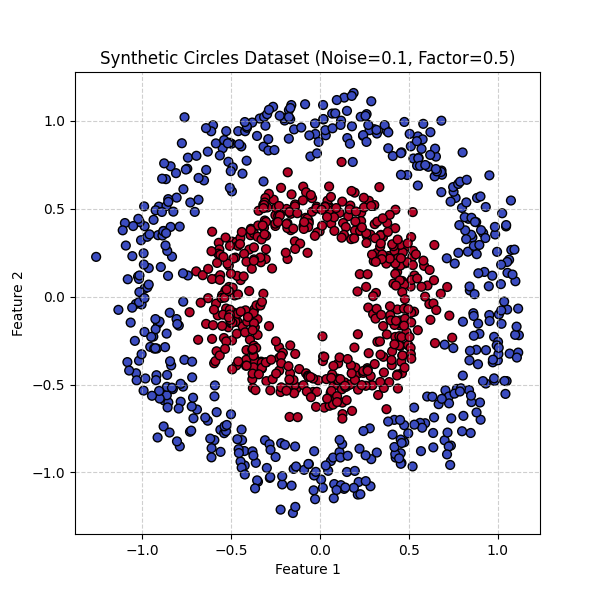
\includegraphics[width=0.6\textwidth]{figures/circle_tests/circles_dataset.png}
     \caption{Plot of the circles dataset}
\end{figure}
\end{center}

\subsection{Stage 1: Optimal Hyperparameters}

\noindent Following the parameter testing from the sine dataset, the following optimal fixed hyperparameters were used for the comparative analysis of the Circle dataset:
\begin{itemize}
    \item \textbf{Quantization Factor:} $Q=10$
    \item \textbf{Parameter Range:} $(-10, 10)$
    \item \textbf{Parameter Fraction ($\text{param\_fraction}$):} $1.0$
    \item \textbf{Target Loss ($L_{\text{target}}$):} $0.0001$
\end{itemize}

\subsection{Stage 2 \& 3: Training and Comparative Analysis}

\noindent The comparison between A* and Gradient Descent is performed over ten independent runs ($n=10$). The analysis utilizes the same statistical methods (Mean Loss with Standard Deviation Shading and Final Loss Box Plot) as used for the previous datasets.

%------------------------------------------------- 1000 iterations -----------------------------------------------

\subsection{Comparison with Gradient Descent: $I_{\text{max}} = 1000$}

\noindent Both A* and GD were executed for a total of $I_{\text{max}}=1000$ steps. The statistical results are summarized in Table \ref{tab:circle_1000_stats}, and the performance trajectory is presented in the following figures.

\begin{center}
\begin{figure}[H]
    \centering
    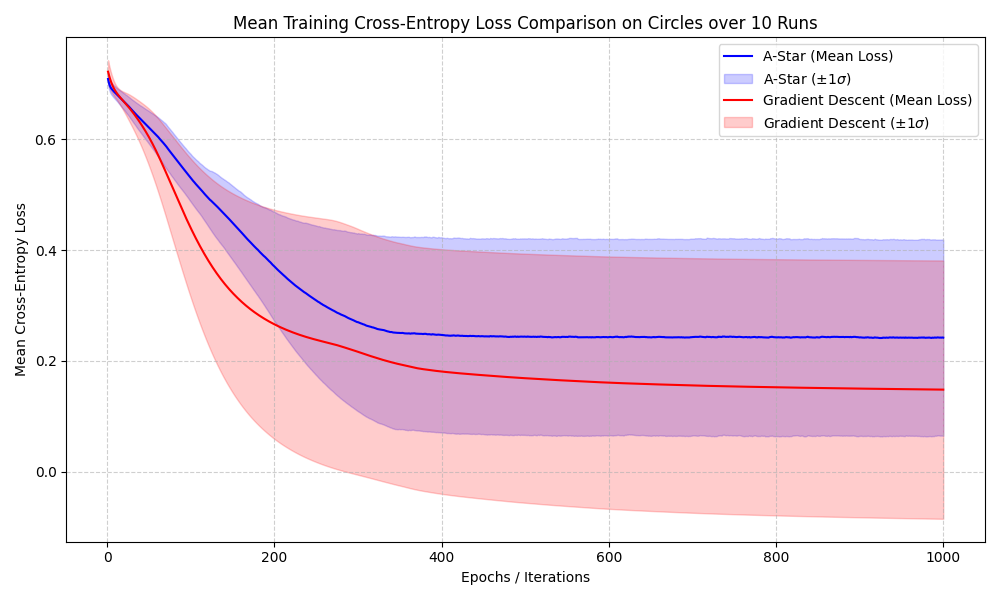
\includegraphics[width=1.0\textwidth]{figures/circle_tests/circle_mean_loss_comparison_with_std_1k.png}
     \caption{Mean Loss Trajectory with Standard Deviation Shading for $I_{\text{max}}=\text{1000}$ Iterations (Circle Dataset). This plot illustrates the average loss over ten independent runs, highlighting convergence and consistency.}
\end{figure}
\end{center}

\begin{center}
\begin{figure}[H]
    \centering
    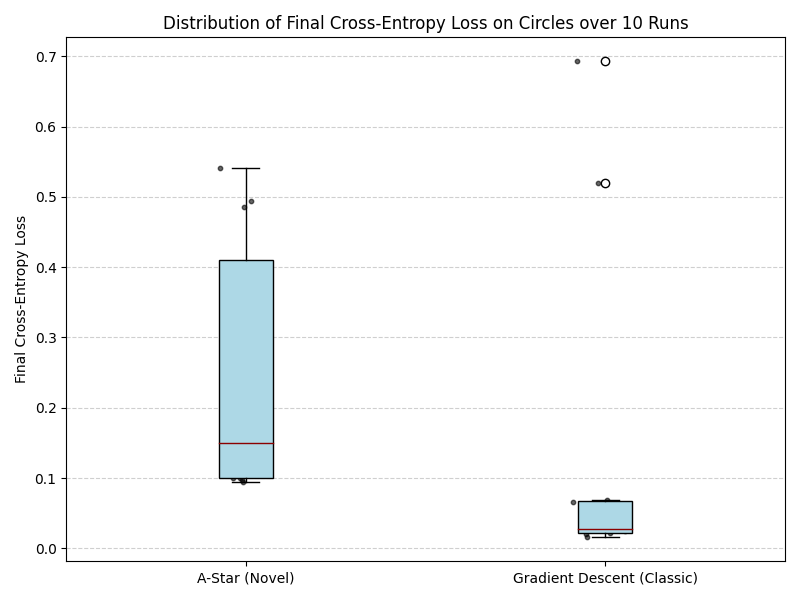
\includegraphics[width=1.0\textwidth]{figures/circle_tests/circle_final_loss_boxplot_1k.png}
     \caption{Final Loss Box Plot for $I_{\text{max}}=\text{1000}$ Iterations (Circle Dataset). This plot summarizes the distribution of the terminal loss values achieved by both search methods.}
\end{figure}
\end{center}

\begin{table}[H]
    \centering
    \caption{Comparative Statistics Over Ten Runs for $I_{\text{max}}=1000$ Iterations (Circle Dataset)}
    \label{tab:circle_1000_stats}
    \begin{tabular}{|l|c|c|}
        \hline
        \textbf{Metric} & \textbf{A* Search (Novel)} & \textbf{Gradient Descent (Classic)} \\
        \hline
        Average Loss ($\bar{L}$) & 0.240124 & \textbf{0.148245} \\
        Median Loss & 0.150237 & \textbf{0.026805} \\
        Standard Deviation ($\sigma$) & \textbf{0.177546} & 0.232974 \\
        Variance ($\sigma^2$) & \textbf{0.031522} & 0.054277 \\
        Minimum Loss ($L_{\min}$) & 0.094537 & \textbf{0.015414} \\
        Maximum Loss ($L_{\max}$) & 0.541776 & \textbf{0.693137} \\
        Average Training Time (s) & 46.892284 & \textbf{6.829286} \\
        \hline
    \end{tabular}
\end{table}

\subsection*{Statistical and Trajectory Analysis}

\noindent \textbf{Performance (Average vs. Median):} For the $1,000$-iteration budget on the Circle dataset, Gradient Descent achieves a superior Average Loss ($\bar{L} = 0.1482$) compared to A* ($\bar{L} = 0.2401$). This difference is even more pronounced in the Median Loss, where GD ($0.0268$) is substantially better than A* ($0.1502$), indicating that GD typically converges to a much stronger solution. GD also found the best-case result, achieving a significantly lower Minimum Loss ($L_{\min} = 0.0154$).

\noindent \textbf{Consistency Trade-off:} The primary performance difference lies in consistency. A* demonstrates superior consistency with a lower Standard Deviation ($\sigma = 0.1775$) and Variance than GD ($\sigma = 0.2330$). This suggests that while GD finds better solutions on average and achieves the absolute minimum, it also produces significantly worse maximum loss results ($L_{\max} = 0.6931$), indicating a higher risk of failed runs or poor local minima entrapment compared to the A* search.

\noindent \textbf{Computational Efficiency:} GD is vastly more efficient, completing the $1,000$ steps in approximately 6.83 seconds, whereas the A* search requires 46.89 seconds due to its high algorithmic overhead.

\noindent \textbf{Conclusion for $I_{\text{max}}=1000$:} Gradient Descent is the performance leader, achieving lower average and minimum loss, but it is less reliable than A* due to its higher variance and susceptibility to poor initializations. A* provides a more consistent, low-variance alternative, albeit at a higher computational cost.


%------------------------------------------------- 2500 iterations -----------------------------------------------

\subsection{Comparison with Gradient Descent: $I_{\text{max}} = 2,500$}

\noindent The comparative study was extended to $I_{\text{max}}=2,500$ steps to evaluate the extended convergence behavior of both methods on the challenging non-linear Circle dataset. The statistical results are summarized in Table \ref{tab:circle_2500_stats}, and the performance trajectory is presented in the following figures.

\begin{center}
\begin{figure}[H]
    \centering
    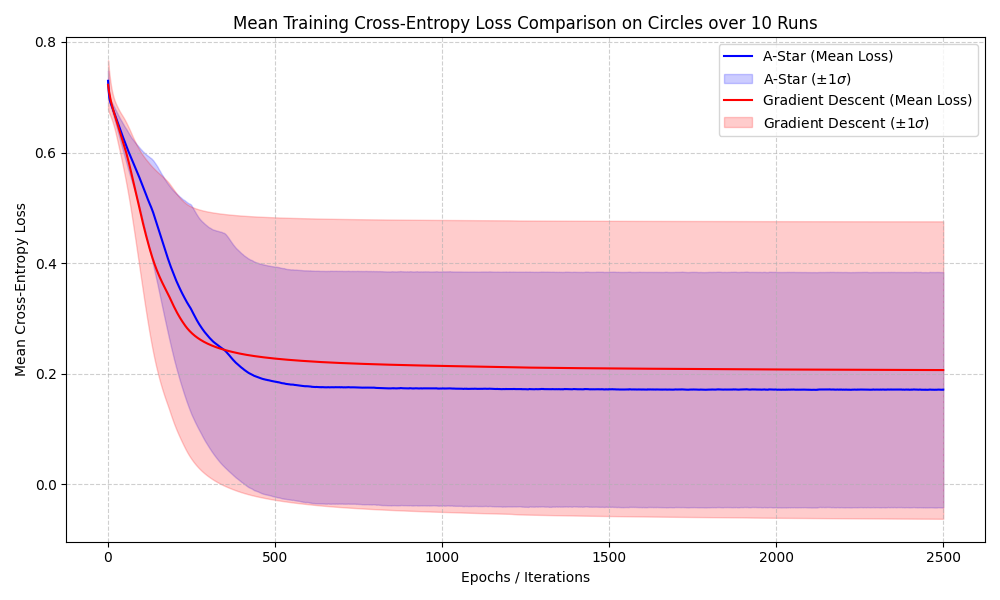
\includegraphics[width=1.0\textwidth]{figures/circle_tests/circle_mean_loss_comparison_with_std_2_5k.png}
     \caption{Mean Loss Trajectory with Standard Deviation Shading for $I_{\text{max}}=\text{2,500}$ Iterations (Circle Dataset). This plot illustrates the average loss over ten independent runs, highlighting convergence and consistency.}
\end{figure}
\end{center}

\begin{center}
\begin{figure}[H]
    \centering
    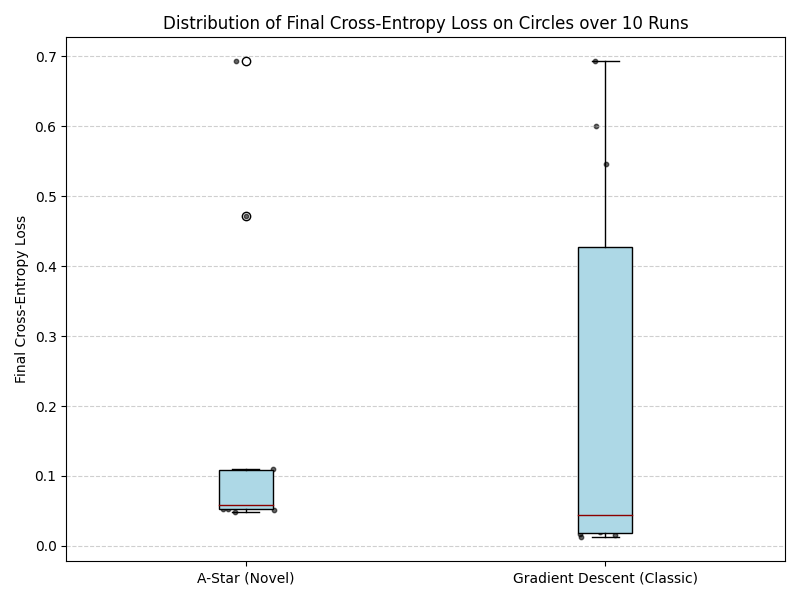
\includegraphics[width=1.0\textwidth]{figures/circle_tests/circle_final_loss_boxplot_2_5k.png}
     \caption{Final Loss Box Plot for $I_{\text{max}}=\text{2,500}$ Iterations (Circle Dataset). This plot summarizes the distribution of the terminal loss values achieved by both search methods.}
\end{figure}
\end{center}

\begin{table}[H]
    \centering
    \caption{Comparative Statistics Over Ten Runs for $I_{\text{max}}=2,500$ Iterations (Circle Dataset)}
    \label{tab:circle_2500_stats}
    \begin{tabular}{|l|c|c|}
        \hline
        \textbf{Metric} & \textbf{A* Search (Novel)} & \textbf{Gradient Descent (Classic)} \\
        \hline
        Average Loss ($\bar{L}$) & \textbf{0.170333} & 0.206681 \\
        Median Loss & 0.058771 & \textbf{0.044057} \\
        Standard Deviation ($\sigma$) & \textbf{0.212892} & 0.268925 \\
        Variance ($\sigma^2$) & \textbf{0.045323} & 0.072320 \\
        Minimum Loss ($L_{\min}$) & 0.048488 & \textbf{0.012027} \\
        Maximum Loss ($L_{\max}$) & \textbf{0.693058} & 0.693147 \\
        Average Training Time (s) & 126.002429 & \textbf{19.916831} \\
        \hline
    \end{tabular}
\end{table}

\subsection*{Statistical and Trajectory Analysis}

\noindent \textbf{Central Tendency Comparison:} With $2,500$ iterations, the performance metrics show a complex trade-off. A* achieves a slightly better Average Loss ($\bar{L}=0.1703$) than GD ($\bar{L}=0.2067$). However, the Median Loss of GD ($0.0441$) is superior to A*'s Median Loss ($0.0588$). This implies that A* is less penalized by outliers (or failed runs) than GD, but GD, when successful, typically finds a marginally better solution.

\noindent \textbf{Best-Case vs. Consistency:} Gradient Descent retains the ability to find the absolute best solutions, achieving a significantly lower Minimum Loss ($L_{\min}=0.0120$) than A* ($L_{\min}=0.0485$). Nevertheless, A* demonstrates superior consistency with a lower Standard Deviation ($\sigma=0.2129$) and Variance ($\sigma^2=0.0453$) compared to GD ($\sigma=0.2689$). Both methods still suffer from the high-variance risk of getting stuck, evidenced by Max Loss values near $0.693$, but A* does so slightly less frequently.

\noindent \textbf{Computational Efficiency:} Gradient Descent remains vastly more efficient, completing $2,500$ steps in approximately 19.92 seconds, while A* requires 126.00 seconds.

\noindent \textbf{Conclusion for $I_{\text{max}}=2,500$:} On the Circle dataset with an extended budget, A* achieves a better overall average loss due to a less frequent occurrence of catastrophic failure runs. However, GD still offers a better median performance and the best minimum loss. The primary distinction is that A* provides a more consistent (lower variance) solution than GD, confirming its robustness in the face of a complex non-linear loss landscape.